\chapter{Diseño del proyecto}\label{cap3}
Conforme a lo visto en el capítulo anterior, el proyecto requiere ser ejecutado de dos formas distintas (ejecución de automatizaciones y portal de usuario), además necesita de una base de datos para persistir los datos de las órdenes de reposición atendidas, catálogos y datos de usuario, también es necesario acceso al sistema de archivo para guardar las capturas de pantalla de las órdenes de reposición enviadas. Es decir, es requerido tener dos ambientes de ejecución, la automatización que será ejecutada exclusivamente en el sistema operativo y la de web, que si bien también estará contenida en el sistema operativo también es previsto que se ejecute parte del sistema en el explorador del usuario.


%===============================================================================
%===============================================================================


\section{Diseño de la arquitectura}
Bourque define la arquitectura de software como:
\begin{quote}
	El conjunto de estructuras necesarias para la comprensión de un sistema en el cual se comprometen elementos de software, relaciones entre ellos y sus propiedades.\cite{SWEBOOK}
\end{quote}
En las últimas décadas la arquitectura de software ha profundizado en el estudio genérico de las estructuras del software, dando lugar a técnicas como Patrones de Diseño y Arquitectura 4+1.
\paragraph{Arquitectura Orientada a Servicios}
\textcolor{red}{Escribir lo que es la arquitectura orientada a servicios (tal vez sería bueno decir porque nos favorece.)}
\paragraph{Patrones de Diseño:} ``Un patrón describe un problema recurrente sobre un ambiente, y entonces describe la técnica que soluciona el problema de forma tal que puede ser utilizado sobre cualquier instancia del problema.''\cite{DesignPatterns}. Esto quiere decir que dados los requerimientos funcionales del sistema es posible analizar la comunicación entre sus distintas partes y de esta forma saber lo patrones que son útiles para dar solución. Los patrones son organizados en tres categorías:
\begin{itemize}
	\item \textbf{Creacionales}: describen la forma en que las entidades (objetos si se utiliza el paradigma orientado a objetos) del sistema son creadas.
	\item \textbf{Estructurales}: describen la organización entre las entidades del sistema.
	\item \textbf{Comportamiento}: describen la comunicación entre entidades del sistema
\end{itemize}
\paragraph{Arquitectura 4+1:} Organiza cada decisión en el diseño del sistema en cuatro partes llamadas vistas, cada vista se encarga de enfocarse en un aspecto del diseño, estas cuatro vistas son unificadas por una cuarta vista de escenarios o casos de uso (ver Figura \ref{fig:dia-arq-4-1}):
\begin{itemize}
	\item \textbf{Vista Lógica}: son las reglas del negocio por las que se rige la operación del usuario final.
	\item \textbf{Vista de Proceso}: refleja concurrencia y sincronización.
	\item \textbf{Vista de Física}: describe las relaciones del software con el hardware.
	\item \textbf{Vista de Desarrollo}: describe la organización estática del software en su ambiente de desarrollo.\cite{ViewModel4plus1}
\end{itemize}

\begin{figure}[h]
\centering
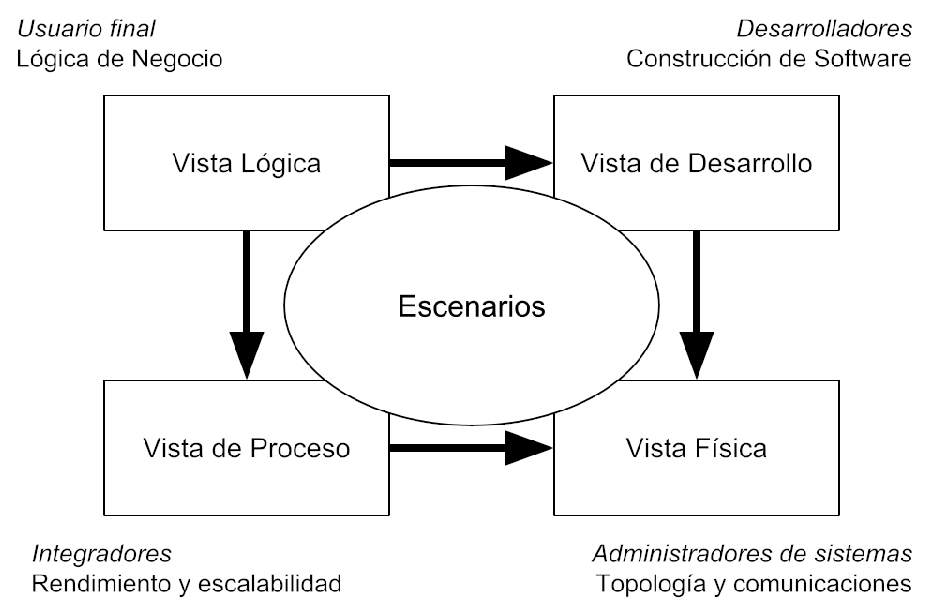
\includegraphics[width=\textwidth]{dia-arq-4-1} 
\caption{Diagrama de arquitectura 4+1.}
\label{fig:dia-arq-4-1}
\end{figure}

Tomando como referencia el modelo ``4+1'' descrito anteriormente, a esta altura se han presentado los escenarios, capítulo \ref{cap2}, y la vista lógica, capítulo \ref{cap1}, a continuación se tratarán temas que conciernen a la vista de Proceso y la vista Física, tocando un poco la vista de Desarrollo, pero esta última será explorada a profundidad en el siguiente capítulo.\\

\textcolor{red}{Esto sería una descripción breve del contenido de cada vista}
\textcolor{blue}{no estoy tan seguro... a ver que sale}

\textcolor{gray}{
Vista de Desarrollo:
Vista de Proceso:
Vista Física:
}


\subsection{Componentes del sistema AutoSA}
El diagrama de componentes sirve para visualizar los componentes en los que se divide el sistema y las interfaces por las cuales se comunican tales componentes, el la Figura \ref{fig:dia-components} se muestra el diagrama de componentes para el sistema AutoSAI.
\begin{figure}[h]
\centering
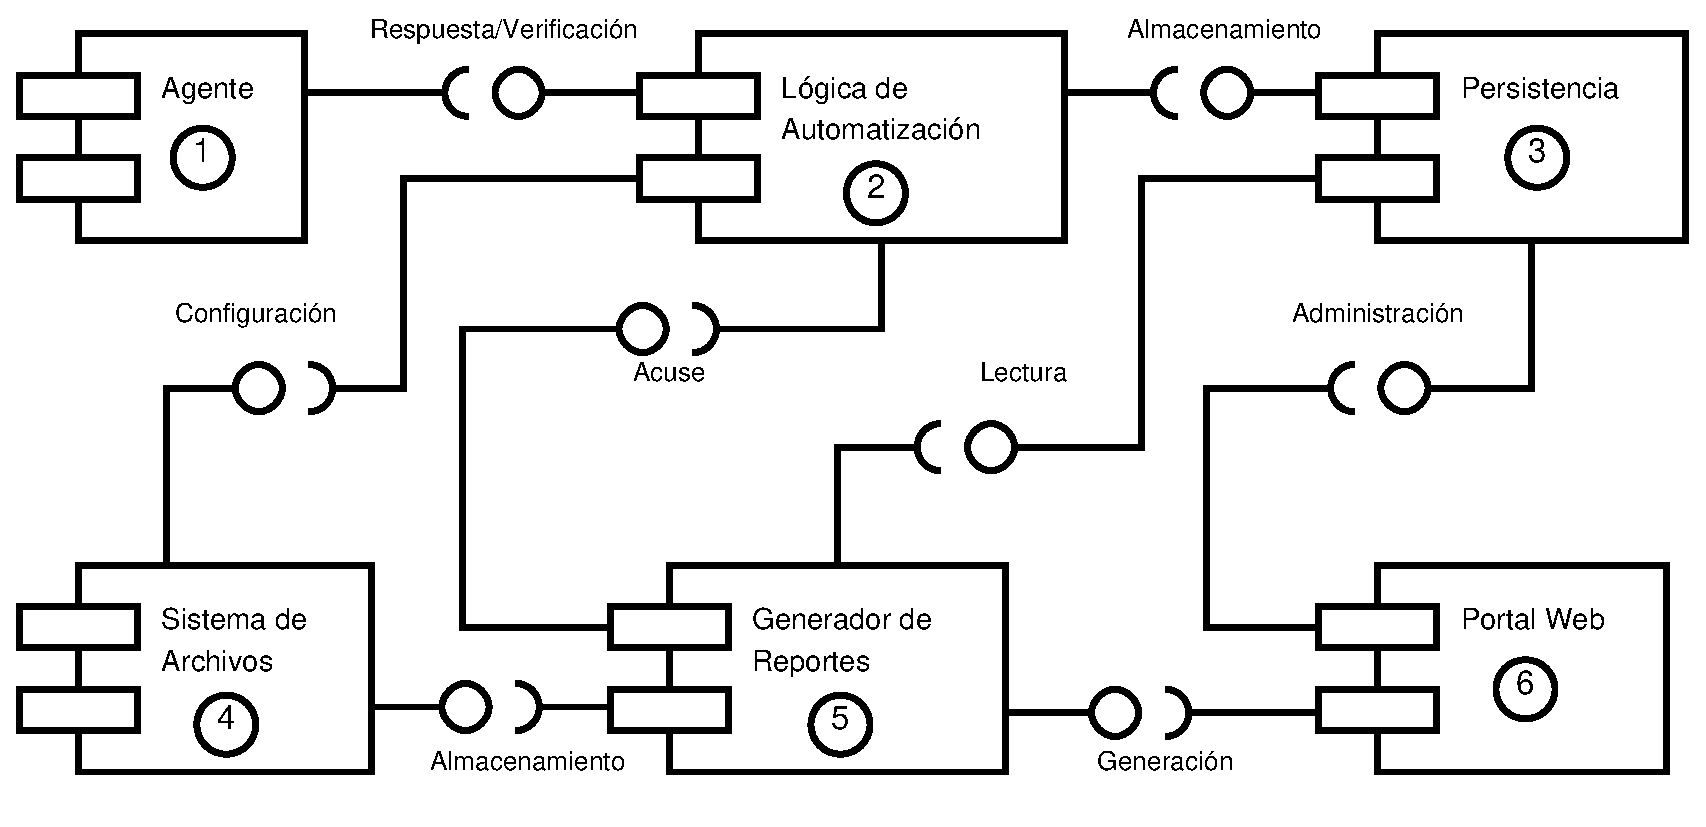
\includegraphics[width=\textwidth]{dia-components}
\caption{Diagrama de componentes.}
\label{fig:dia-components}
\end{figure}

A continuación se muestran las interfaces mediante las cuales los componentes ofrecen conjuntos de operaciones.

\subsubsection{Persistencia}
El componente de persistencia está basado en el patrón de diseño \textit{DAO}\footnote{Ver apéndice \ref{sec-dao}}\footnote{En adelante se utilizará \textbf{DAO} para hacer referencia al patrón y la instancia (objeto) del patrón.} para controlar el acceso a la base de datos.\\
El componente de persistencia de el proyecto AutoSA presenta las siguientes interfaces de búsqueda y almacenamiento:
\paragraph{Almacenamiento\\}
Conjunto de operaciones diseñadas para responder a las necesidades de almacenamiento en los flujos para responder y verificar órdenes de reposición\footnote{Ver casos de uso \ref{cu-contestar}, \ref{cu-guardar-nueva}, \ref{cu-responder-orden}, \ref{cu-enviar-orden} y \ref{cu-actualizar-estatus-sa}.}:
	\vspace{5mm}\\
	\begin{tabular}{|p{\dimexpr.2\textwidth}|p{\dimexpr.8\textwidth-4\tabcolsep}|}
		\hline
		\textbf{Identificador}	& \textbf{guardar-nueva} \\
		\hline
		\hline
		\textbf{Descripción}	& Inserta una nueva orden de reposición en la base de datos.\\
		\hline
		\textbf{Parámetros} 	& \textbullet\, Mapa con los datos de la orden de reposición.\\
		\hline
		\textbf{Resultado}		& No ofrece resultado.\\
		\hline
	\end{tabular}
	\vspace{5mm}\\
	\textcolor{red}{Karla, pienso que hacer diagramas de secuencia como el de la figura \ref{fig:dia-seq-store-save-new} es muy simple, pero no sé si aún así sea necesario ¿sería posible nada más incluir los diagramas de secuencia no triviales?\\\\}
	\begin{figure}[h]
		\centering
		\includegraphics[scale=0.4]{dia-seq-store-save-new}
		\caption{Diagrama de secuencia de la operación guardar-nueva de la interfaz Almacenamiento.}
		\label{fig:dia-seq-store-save-new}
	\end{figure}
%	\vspace{5mm}\\
	\begin{tabular}{|p{\dimexpr.2\textwidth}|p{\dimexpr.8\textwidth-4\tabcolsep}|}
		\hline
		\textbf{Identificador}	& \textbf{cambiar-estado} \\
		\hline
		\hline
		\textbf{Descripción}	& Cambia el estado de atención de una orden de reposición. \\
		\hline
		\multirow{2}{*}{\textbf{Parámetros}}	& \textbullet\, Número de orden de reposición.\\
												& \textbullet\, Estado.\\
		\hline
		\textbf{Resultado}		& No ofrece resultado.\\
		\hline
	\end{tabular}
	\vspace{5mm}\\
	\begin{tabular}{|p{\dimexpr.2\textwidth}|p{\dimexpr.8\textwidth-4\tabcolsep}|}
		\hline
		\textbf{Identificador}	& \textbf{guardar-respuesta}\\
		\hline
		\hline
		\textbf{Descripción}	& Guarda los datos de los formularios de la pantalla de respuesta de las órdenes de reposición.\\
		\hline
		\multirow{2}{*}{\textbf{Parámetros}}	& \textbullet\, Número de orden de reposición.\\
												& \textbullet\, Mapa con los datos de los formularios.\\
		\hline
		\textbf{Resultado}		& No ofrece resultado.\\
		\hline
	\end{tabular}
	\vspace{5mm}\\
	\begin{tabular}{|p{\dimexpr.2\textwidth}|p{\dimexpr.8\textwidth-4\tabcolsep}|}
		\hline
		\textbf{Identificador}	& \textbf{guardar-folio-acuse}\\
		\hline
		\hline
		\textbf{Descripción}	& Guarda el folio de acuse de envío de la orden de reposición.\\
		\hline
		\multirow{2}{*}{\textbf{Parámetros}} 	& \textbullet\, Número de orden de reposición.\\
												& \textbullet\, Folio de acuse de envío.\\
		\hline
		\textbf{Resultado}		& No ofrece resultado.\\
		\hline
	\end{tabular}
	\vspace{5mm}\\
	\begin{tabular}{|p{\dimexpr.2\textwidth}|p{\dimexpr.8\textwidth-4\tabcolsep}|}
		\hline
		\textbf{Identificador}	& \textbf{actualizar-estado-sa}\\
		\hline
		\hline
		\textbf{Descripción}	& Actualiza el estado de atención SA a \textbf{cancelada} de las ordenes de reposición recibidas.\\
		\hline
		\textbf{Parámetros} 	& \textbullet\, Lista con los números de las órdenes de reposición.\\
		\hline
		\textbf{Resultado}		& El número de órdenes de reposición actualizadas.\\
		\hline
	\end{tabular}
	\vspace{5mm}\\
	\begin{tabular}{|p{\dimexpr.2\textwidth}|p{\dimexpr.8\textwidth-4\tabcolsep}|}
		\hline
		\textbf{Identificador}	& \textbf{registrar-evento}\\
		\hline
		\hline
		\textbf{Descripción}	& Registra en la base de datos un evento que ocurre durante los procesos automatizados, el evento puede ser de carácter informativo o de error.\\
		\hline
		\multirow{2}{*}{\textbf{Parámetros}}	& \textbullet\, Tipo de evento.\\
												& \textbullet\, Mapa con la descripción del evento.\\
		\hline
		\textbf{Resultado}		& No ofrece resultado.\\
		\hline
	\end{tabular}
	\vspace{5mm}

\paragraph{Lectura\\}
Conjunto de operaciones diseñadas para las necesidades de lectura de órdenes de reposición en los flujos para responder y verificar órdenes de reposición\footnote{Ver casos de uso \ref{cu-contestar}, \ref{cu-enviar-orden} y \ref{cu-generar-acuse}.}:
	\vspace{5mm}\\
	\begin{tabular}{|p{\dimexpr.2\textwidth}|p{\dimexpr.8\textwidth-4\tabcolsep}|}
		\hline
		\textbf{Identificador}	& \textbf{siguiente-orden-contestar}\\
		\hline
		\hline
		\textbf{Descripción}	& Entrega un mapa con los datos de la primera orden de reposición encontrada con estado \textbf{Nueva}.\\
		\hline
		\textbf{Parámetros} 	& \textbullet\, \textit{No tiene parámetros}.\\
		\hline
		\textbf{Resultado}		& Un mapa con los datos de la primera orden de reposición encontrada con estado \textbf{Nueva}. En caso de no existir tal orden regresa un mapa vacío.\\
		\hline
	\end{tabular}
	\vspace{5mm}\\
	\begin{tabular}{|p{\dimexpr.2\textwidth}|p{\dimexpr.8\textwidth-4\tabcolsep}|}
		\hline
		\textbf{Identificador}	& \textbf{siguiente-orden-enviar}\\
		\hline
		\hline
		\textbf{Descripción}	& Entrega un mapa con los datos de la primera orden de reposición encontrada con estado \textbf{Contestada}.\\
		\hline
		\textbf{Parámetros} 	& \textbullet\, \textit{No tiene parámetros}.\\
		\hline
		\textbf{Resultado}		& Un mapa con los datos de la primera orden de reposición encontrada con estado \textbf{Contestada}. En caso de no existir tal orden regresa un mapa vacío.\\
		\hline
	\end{tabular}
	\vspace{5mm}\\
	\begin{tabular}{|p{\dimexpr.2\textwidth}|p{\dimexpr.8\textwidth-4\tabcolsep}|}
		\hline
		\textbf{Identificador}	& \textbf{obtener-datos-acuse}\\
		\hline
		\hline
		\textbf{Descripción}	& Obtiene los datos de una orden de reposición necesarios para generar el documento de acuse de envío.\\
		\hline
		\textbf{Parámetros}		& \textbullet\, Número de orden de reposición.\\
		\hline
		\textbf{Resultado}		& Un mapa con los datos de la orden de reposición. En caso de no existir tal orden regresa un mapa vacío.\\
		\hline
	\end{tabular}
	\vspace{5mm}

\paragraph{Administración\\}
Son las operaciones que permiten modificar datos específicos de las órdenes de reposición contenidas en la base de datos, también ofrece la actualización masiva de catálogos\footnote{Ver casos de uso \ref{cu-entrar-web}, \ref{cu-generar-reporte}, \ref{cu-actualizar-catalogo}, \ref{cu-buscar}, \ref{cu-visualizar} y \ref{cu-editar}.}).
	\vspace{5mm}\\
	\begin{tabular}{|p{\dimexpr.2\textwidth}|p{\dimexpr.8\textwidth-4\tabcolsep}|}
		\hline
		\textbf{Identificador}	& \textbf{buscar-credenciales}\\
		\hline
		\hline
		\textbf{Descripción}	& Busca las credenciales del usuario.\\
		\hline
		\textbf{Parámetros}		& \textbullet\, Identificador de usuario.\\
		\hline
		\textbf{Resultado}		& Un mapa con las credenciales del usuario.\\
		\hline
	\end{tabular}
	\vspace{5mm}\\
	\begin{tabular}{|p{\dimexpr.2\textwidth}|p{\dimexpr.8\textwidth-4\tabcolsep}|}
		\hline
		\textbf{Identificador}	& \textbf{extraer-reporte}\\
		\hline
		\hline
		\textbf{Descripción}	& Ejecuta la búsqueda necesaria para extraer los datos del reporte indicado.\\
		\hline
		\multirow{2}{*}{\textbf{Parámetros}}	& \textbullet\, Tipo de reporte.\\
												& \textbullet\, Mapa con los parámetros del filtro de búsqueda.\\
		\hline
		\textbf{Resultado}		& Un listado con los datos del reporte.\\
		\hline
	\end{tabular}
	\vspace{5mm}\\
	\begin{tabular}{|p{\dimexpr.2\textwidth}|p{\dimexpr.8\textwidth-4\tabcolsep}|}
		\hline
		\textbf{Identificador}	& \textbf{actualizar-catalogo}\\
		\hline
		\hline
		\textbf{Descripción}	& Actualiza la información del catálogo indicado.\\
		\hline
		\multirow{2}{*}{\textbf{Parámetros}}	& \textbullet\, Identificador del catálogo.\\
												& \textbullet\, Listado con los datos del catálogo.\\
		\hline
		\textbf{Resultado}		& El número de los registros insertados en el catálogo.\\
		\hline
	\end{tabular}
	\vspace{5mm}\\
	\begin{tabular}{|p{\dimexpr.2\textwidth}|p{\dimexpr.8\textwidth-4\tabcolsep}|}
		\hline
		\textbf{Identificador}	& \textbf{buscar-ordenes}\\
		\hline
		\hline
		\textbf{Descripción}	& Busca órdenes de reposición que cumplan con el filtro de búsqueda indicado.\\
		\hline
		\textbf{Parámetros}		& \textbullet\, Mapa con el filtro de búsqueda.\\
		\hline
		\textbf{Resultado}		& Un listado con las órdenes de reposición encontradas.\\
		\hline
	\end{tabular}
	\vspace{5mm}\\
	\begin{tabular}{|p{\dimexpr.2\textwidth}|p{\dimexpr.8\textwidth-4\tabcolsep}|}
		\hline
		\textbf{Identificador}	& \textbf{buscar-orden}\\
		\hline
		\hline
		\textbf{Descripción}	& Busca una orden de reposición por el número de orden.\\
		\hline
		\textbf{Parámetros}		& \textbullet\, Número de orden de reposición.\\
		\hline
		\textbf{Resultado}		& La orden de reposición encontrada. En caso de no encontrar la orden se regresa un identificador vacío.\\
		\hline
	\end{tabular}
	\vspace{5mm}\\
	\begin{tabular}{|p{\dimexpr.2\textwidth}|p{\dimexpr.8\textwidth-4\tabcolsep}|}
		\hline
		\textbf{Identificador}	& \textbf{actualizar-orden}\\
		\hline
		\hline
		\textbf{Descripción}	& Actualiza los datos de orden de reposición.\\
		\hline
		\multirow{2}{*}{\textbf{Parámetros}}	& \textbullet\, Número de orden.\\
												& \textbullet\, Mapa con los datos actualizados.\\
		\hline
		\textbf{Excepciones}	& Error si la orden de reposición no se encuentra registrada en la base de datos.\\
		\hline
	\end{tabular}
	\vspace{5mm}

\subsubsection{Sistema de archivos}
El componente Sistema de archivos es el único que se comunica con el sistema de archivos del sistema operativo\footnote{En este documento se utilizará de forma indistinta el término Sistema de archivos para referirse tanto al componente del sistema AutoSA como al propio del sistema operativo.}, tiene la función de realizar lectura de archivos de configuración, guardar los acuses de envío  y los reportes de las ordenes de reposición.\\
Este componente también está diseñado siguiendo el patrón DAO\footnote{Ver apéndice \ref{sec-dao}}.
\paragraph{Configuración\\}
Da la configuración contenida en archivos de propiedades contenidas en el mismo sistema de archivos.
	\vspace{5mm}\\
	\begin{tabular}{|p{\dimexpr.2\textwidth}|p{\dimexpr.8\textwidth-4\tabcolsep}|}
		\hline
		\textbf{Identificador}	& \textbf{obtener-propiedad}\\
		\hline
		\hline
		\textbf{Descripción}	& Obtiene una propiedad de los archivos de configuración.\\
		\hline
		\textbf{Parámetros}		& \textbullet\, Identificador de la propiedad.\\
		\hline
		\textbf{Resultado}		& El valor de la propiedad. Si no existe la propiedad regresa la cadena vacía.\\
		\hline
	\end{tabular}
	\vspace{5mm}
\paragraph{Almacenamiento\\}
Almacena archivos (reportes y acuses de envío) en el sistema de archivos.
	\vspace{5mm}\\
	\begin{tabular}{|p{\dimexpr.2\textwidth}|p{\dimexpr.8\textwidth-4\tabcolsep}|}
		\hline
		\textbf{Identificador}	& \textbf{guardar-archivo}\\
		\hline
		\hline
		\textbf{Descripción}	& Guarda un archivo en el sistema de archivos.\\
		\hline
		\multirow{2}{*}{\textbf{Parámetros}}	& \textbullet\, Archivo.\\
												& \textbullet\, Ruta del archivo.\\
		\hline
		\textbf{Resultado}		& No ofrece resultado.\\
		\hline
	\end{tabular}
	\vspace{5mm}

\subsubsection{Generador de reportes}
El generador de reportes, como su nombre lo indica, tiene la función de generar documentos y reportes con los datos de las órdenes de reposición almacenados en la base de datos. 
\paragraph{Acuse\\} Genera el documento con el acuse de envío.
	\vspace{5mm}\\
	\begin{tabular}{|p{\dimexpr.2\textwidth}|p{\dimexpr.8\textwidth-4\tabcolsep}|}
		\hline
		\textbf{Identificador}	& \textbf{generar-acuse-envio}\\
		\hline
		\hline
		\textbf{Descripción}	& Genera el acuse de envío para la orden de reposición especificada. Utiliza el componente de persistencia para obtener los datos de la orden.\\
		\hline
		\textbf{Parámetros}		& \textbullet\, Número de la orden de reposición.\\
		\hline
		\textbf{Resultado}		& La ruta en el sistema de archivos donde ha sido depositado el acuse de envío.\\
		\hline
	\end{tabular}
	\vspace{5mm}

\paragraph{Generación\\} Genera reportes con los datos de las órdenes de reposición almacenados en la base de datos.
	\vspace{5mm}\\
	\begin{tabular}{|p{\dimexpr.2\textwidth}|p{\dimexpr.8\textwidth-4\tabcolsep}|}
		\hline
		\textbf{Identificador}	& \textbf{generar-reporte-ordenes}\\
		\hline
		\hline
		\textbf{Descripción}	& Genera el reporte del tipo indicado y entre el rango de fechas dado.\\
		\hline
		\multirow{3}{*}{\textbf{Parámetros}}	& \textbullet\, Tipo de reporte.\\
												& \textbullet\, Fecha inicial.\\
												& \textbullet\, Fecha final.\\
		\hline
		\textbf{Resultado}		& La ruta en el sistema de archivos donde ha sido depositado el reporte generado.\\
		\hline
	\end{tabular}
	\vspace{5mm}

\subsubsection{Lógica de automatización}
La función de este componente es de ejecutar las reglas de negocio necesarias para en los flujos de los procesos de automatización.  
\paragraph{Respuesta\\}
Provee el acceso a las reglas de negocio del proceso de respuesta de órdenes de reposición (ver caso de uso \ref{cu-contestar}).
	\vspace{5mm}\\
	\begin{tabular}{|p{\dimexpr.2\textwidth}|p{\dimexpr.8\textwidth-4\tabcolsep}|}
		\hline
		\textbf{Identificador}	& \textbf{guardar-orden-nueva}\\
		\hline
		\hline
		\textbf{Descripción}	& Guarda un listado de nuevas órdenes de reposición.\\
		\hline
		\textbf{Parámetros}		& \textbullet\, Listado de mapas, cada mapa contiene los datos de una ordenes de reposición.\\
		\hline
		\textbf{Resultado}		& No ofrece resultado.\\
		\hline
	\end{tabular}
	\vspace{5mm}\\
	\begin{tabular}{|p{\dimexpr.2\textwidth}|p{\dimexpr.8\textwidth-4\tabcolsep}|}
		\hline
		\textbf{Identificador}	& \textbf{obtener-datos-respuesta}\\
		\hline
		\hline
		\textbf{Descripción}	& Da los datos necesarios para llenar los formularios para contestar una orden de reposición en SA.\\
		\hline
		\textbf{Parámetros}		& \textbullet\, Mapa con los datos de la orden para contestar.\\
		\hline
		\textbf{Resultado}		& Mapa con la información para llenar los formularios para contestar la orden de reposición.\\
		\hline
	\end{tabular}
	\vspace{5mm}\\
	\begin{tabular}{|p{\dimexpr.2\textwidth}|p{\dimexpr.8\textwidth-4\tabcolsep}|}
		\hline
		\textbf{Identificador}	& \textbf{actualizar-orden-contestada}\\
		\hline
		\hline
		\textbf{Descripción}	& Actualiza los datos guardados de la orden de reposición con los datos de la respuesta en SA. Utiliza el componente de persistencia para actualizar los datos.\\
		\hline
		\multirow{2}{*}{\textbf{Parámetros}}	& \textbullet\, Número de orden.\\
												& \textbullet\, Mapa con los datos para guardar.\\
		\hline
		\textbf{Resultado}		& No ofrece resultado.\\
		\hline
	\end{tabular}
	\vspace{5mm}\\
	\begin{tabular}{|p{\dimexpr.2\textwidth}|p{\dimexpr.8\textwidth-4\tabcolsep}|}
		\hline
		\textbf{Identificador}	& \textbf{guardar-orden-enviada}\\
		\hline
		\hline
		\textbf{Descripción}	& Actualiza los datos guardados de la orden de reposición con los datos de la pantalla de envío de SA. Utiliza el componente de persistencia para actualizar los datos.\\
		\hline
		\multirow{2}{*}{\textbf{Parámetros}}	& \textbullet\, Número de orden.\\
												& \textbullet\, Mapa con los datos para guardar.\\
		\hline
		\textbf{Resultado}		& No ofrece resultado.\\
		\hline
	\end{tabular}
	\vspace{5mm}\\
	\begin{tabular}{|p{\dimexpr.2\textwidth}|p{\dimexpr.8\textwidth-4\tabcolsep}|}
		\hline
		\textbf{Identificador}	& \textbf{obtener-acuse-envio}\\
		\hline
		\hline
		\textbf{Descripción}	& Solicita la generación de el acuse de envío al componente de reportes y almacena el documento en el sistema de archivos utilizando el componente de sistema de archivos.\\
		\hline
		\textbf{Parámetros}		& \textbullet\, Número de orden.\\
		\hline
		\textbf{Resultado}		& No ofrece resultado.\\
		\hline
	\end{tabular}
	\vspace{5mm}
\paragraph{Verificación\\}
Provee el acceso a las reglas de negocio del proceso de verificación de órdenes de reposición canceladas.
	\vspace{5mm}\\
	\begin{tabular}{|p{\dimexpr.2\textwidth}|p{\dimexpr.8\textwidth-4\tabcolsep}|}
		\hline
		\textbf{Identificador}	& \textbf{obtener-rango-fechas-verificar}\\
		\hline
		\hline
		\textbf{Descripción}	& Obtiene el rango de fechas para ingresar en el formulario de búsqueda de SA. El número de días que comprende el rango se obtiene utilizando el componente de Sistema de archivos.\\
		\hline
		\textbf{Parámetros}		& \textbullet\, No tiene parámetros.\\
		\hline
		\textbf{Resultado}		& El número de días para el rango de búsqueda.\\
		\hline
	\end{tabular}
	\vspace{5mm}\\
	\begin{tabular}{|p{\dimexpr.2\textwidth}|p{\dimexpr.8\textwidth-4\tabcolsep}|}
		\hline
		\textbf{Identificador}	& \textbf{actualizar-estado-sa}\\
		\hline
		\hline
		\textbf{Descripción}	& Actualiza el estado SA de las órdenes de reposición recibidas a. \textbf{Cancelada}. Utiliza el componente de persistencia para la actualización de datos.\\
		\hline
		\textbf{Parámetros}		& \textbullet\, Listado con los números de las órdenes de reposición canceladas.\\
		\hline
		\textbf{Resultado}		& El número de órdenes de reposición actualizadas.\\
		\hline
	\end{tabular}
	\vspace{5mm}

\subsubsection{Robot}
El componente que contiene y ejecuta las rutinas de automatización, esto es mediante una interfaz con el usuario en la cual puede seleccionar el proceso a ser ejecutado. No ofrece interfaces a los demás componentes, consume exclusivamente el componente de Lógica de automatización.\\

\subsubsection{Portal Web}
Es componente que ofrece al usuario las funcionalidades de una interfaz web, está diseñado siguiendo el patrón MVC\footnote{Ver sección \ref{sec-mvc}}. Utiliza el componente de persistencia como el modelo, mientras que la vista se toma en dos partes: las pantallas que se muestran al usuario y los reportes, para esta última toma las funciones del componente de Generación de reportes y Sistema de archivos.\\
No ofrece interfaces a los demás componentes, al igual que el componente Robot.

\subsection{Solución a casos de uso}
A continuación se presentan las soluciones a los casos de uso utilizando los componentes descritos en la sección anterior, para este fin se utilizan diagramas de secuencia UML\footnote{Ver sección \ref{sec-uml-seq}.}
\textcolor{red}{Karla, en esta sección pretendo describir los flujos entre componentes que solucionan cada caso de uso.}

\subsubsection{Contestar órdenes}
\textcolor{red}{
	Esta es la muestra de como se presenta el flujo entre componentes para solucionar el caso de uso. Básicamente consiste en mostrar un diagrama de secuencia.\\
	Aún no se hace mención a lenguajes, frameworks o tecnologías específicas, todo eso será en el siguiente capítulo.
}
Ver sección \ref{cu-contestar}.\\
\begin{figure}[h]
	\centering
	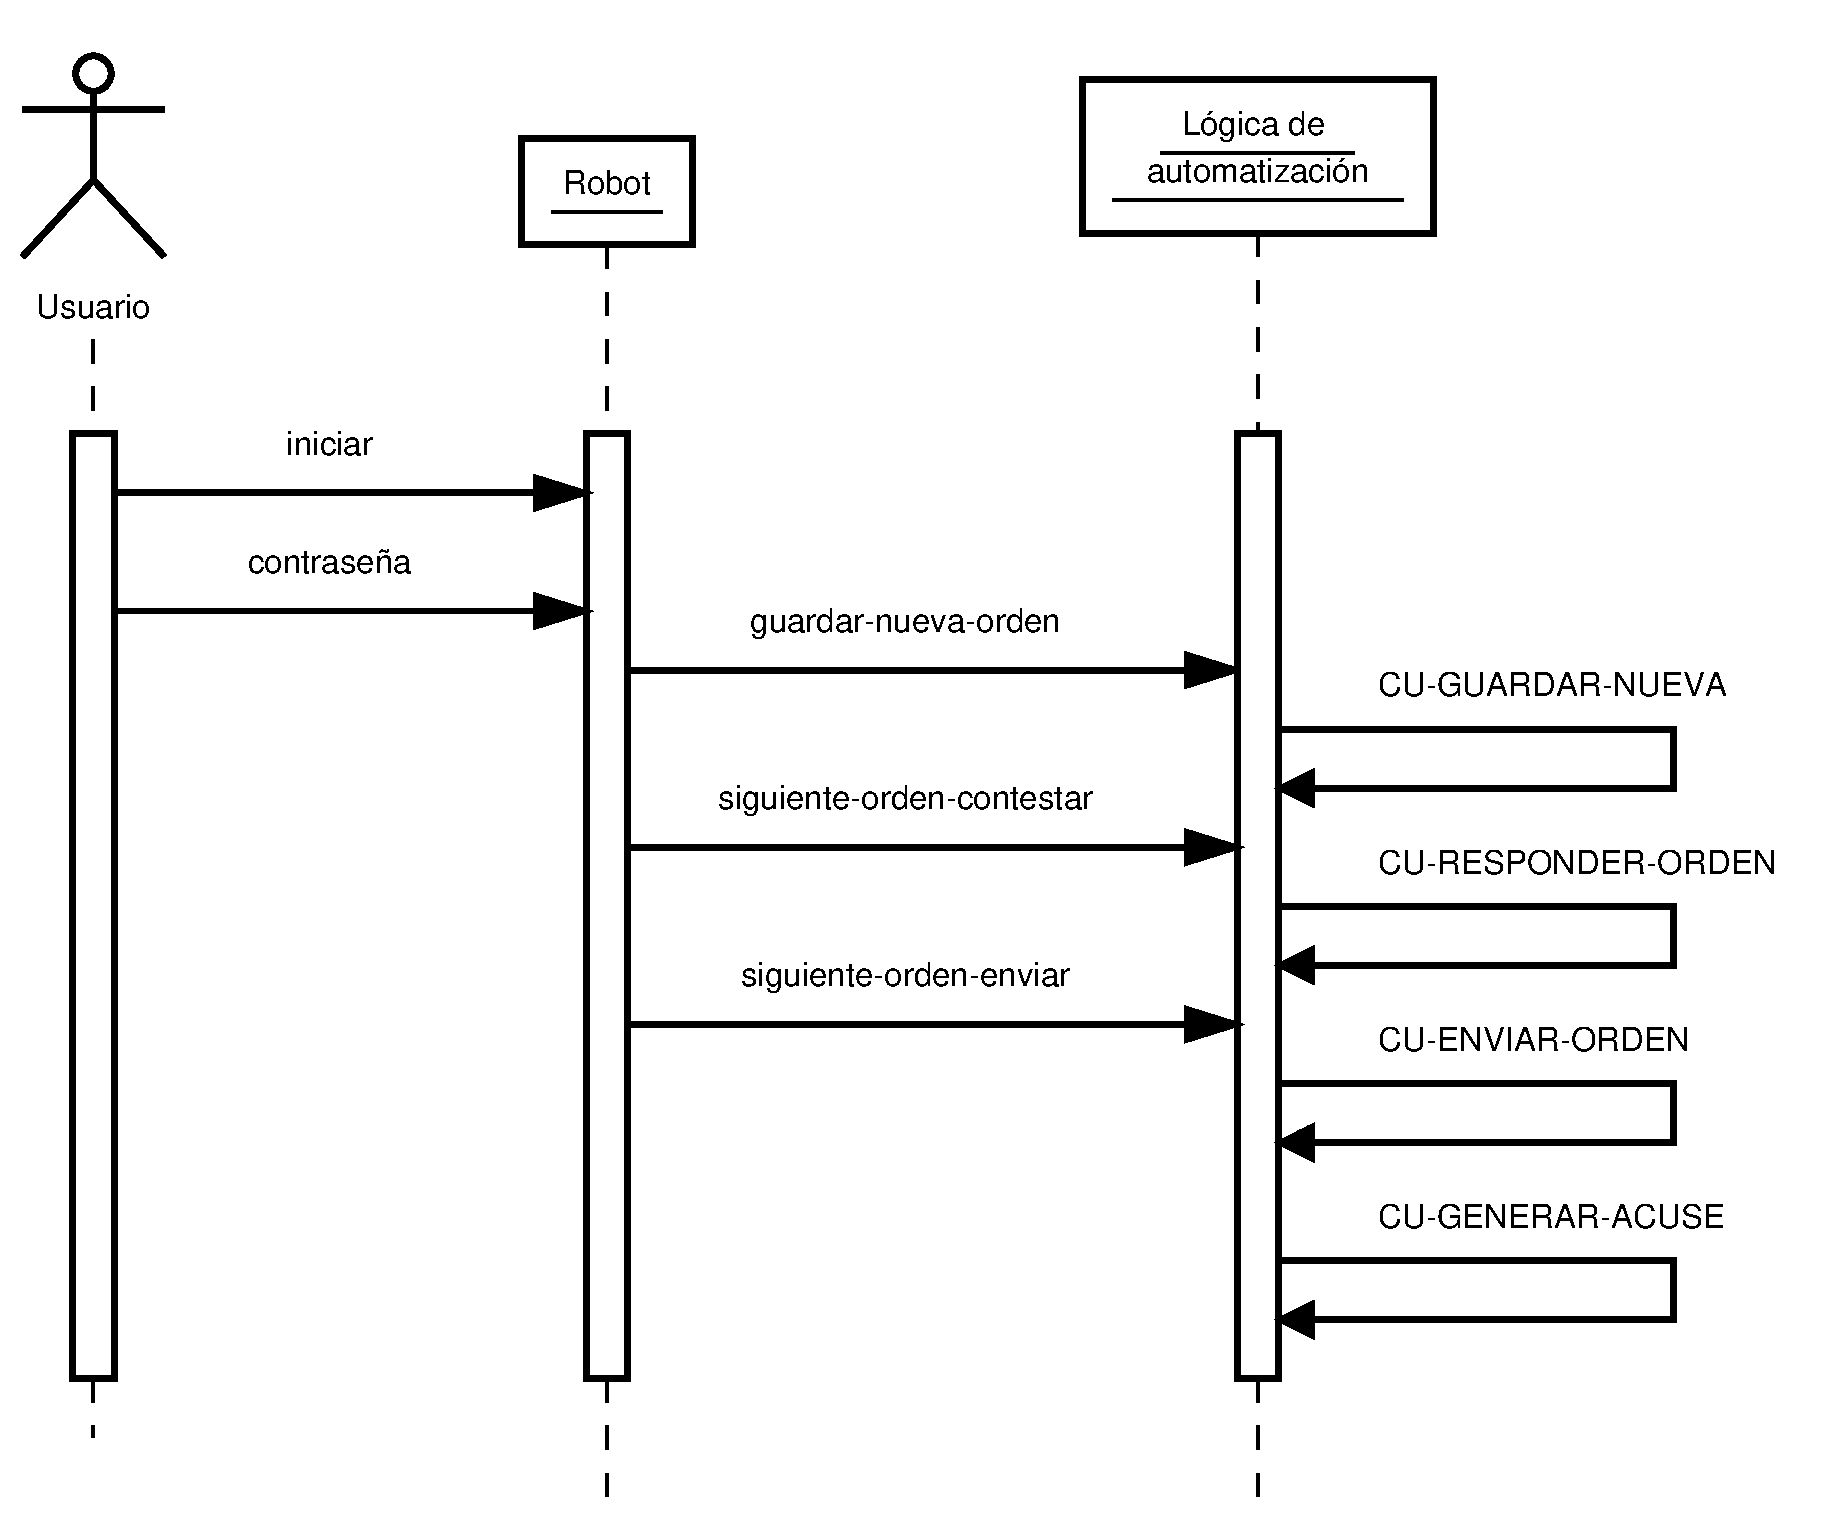
\includegraphics[width=\textwidth]{dia-seq-cu-contestar}
	\caption{Diagrama de secuencia caso de uso contestar órdenes.}
	\label{fig:dia-seq-cu-contestar}
\end{figure}
\iffalse
\subsubsection{Guardar nueva orden}
Ver sección \ref{cu-contestar}.\\
\begin{figure}[h]
	\centering
	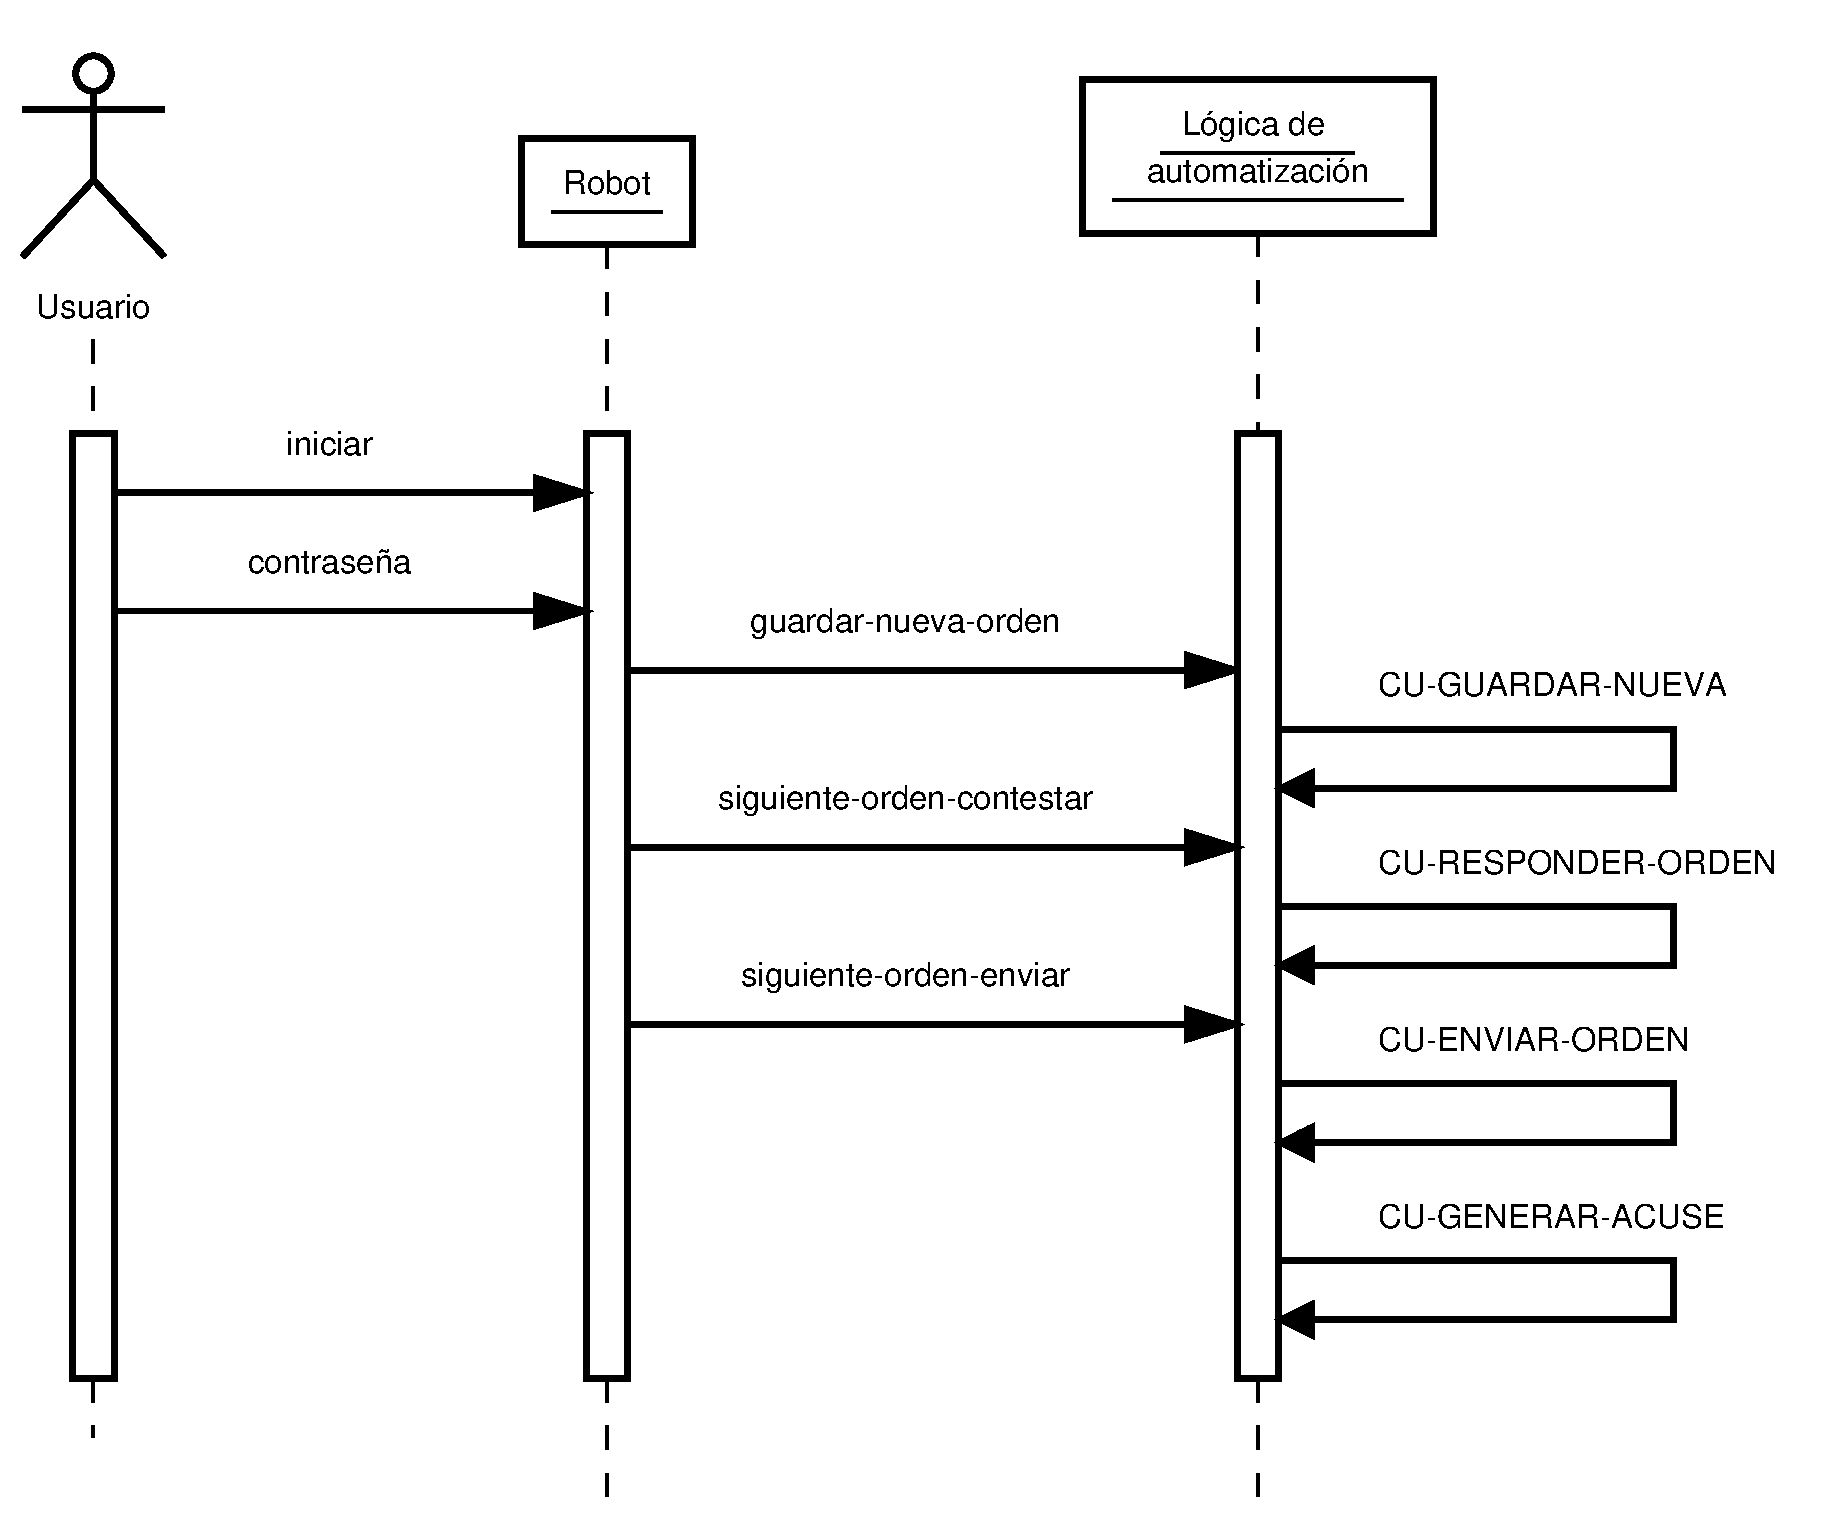
\includegraphics[width=\textwidth]{dia-seq-cu-contestar}
	\caption{Diagrama de secuencia caso de uso contestar órdenes.}
	\label{fig:dia-seq-cu-contestar}
\end{figure}
\subsubsection{Responder orden}
Ver sección \ref{cu-contestar}.\\
\begin{figure}[h]
	\centering
	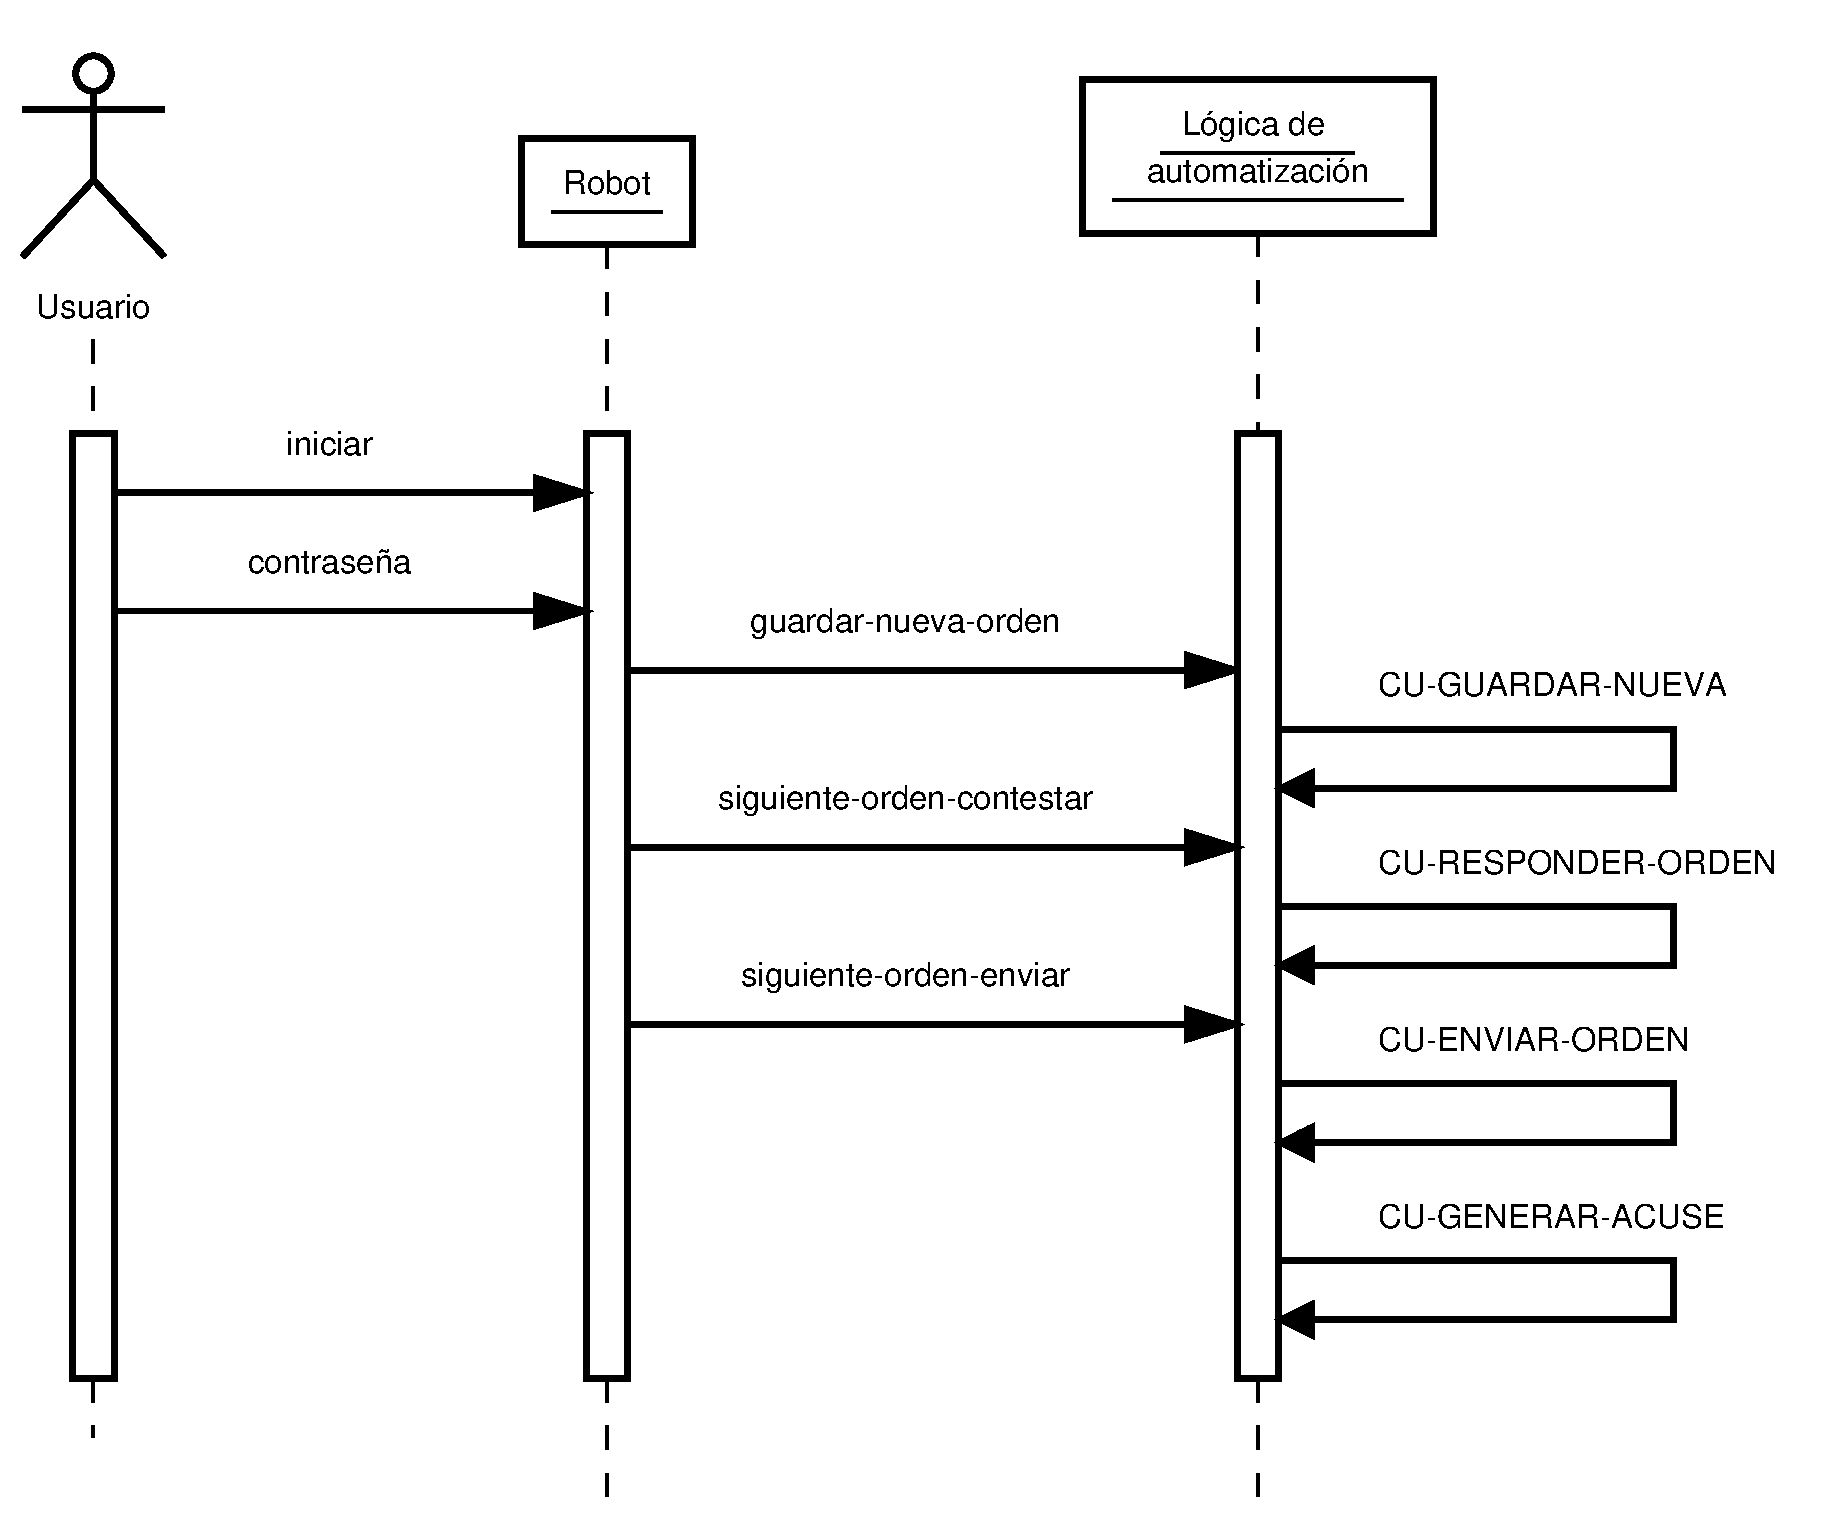
\includegraphics[width=\textwidth]{dia-seq-cu-contestar}
	\caption{Diagrama de secuencia caso de uso contestar órdenes.}
	\label{fig:dia-seq-cu-contestar}
\end{figure}
\subsubsection{Enviar orden}
Ver sección \ref{cu-contestar}.\\
\begin{figure}[h]
	\centering
	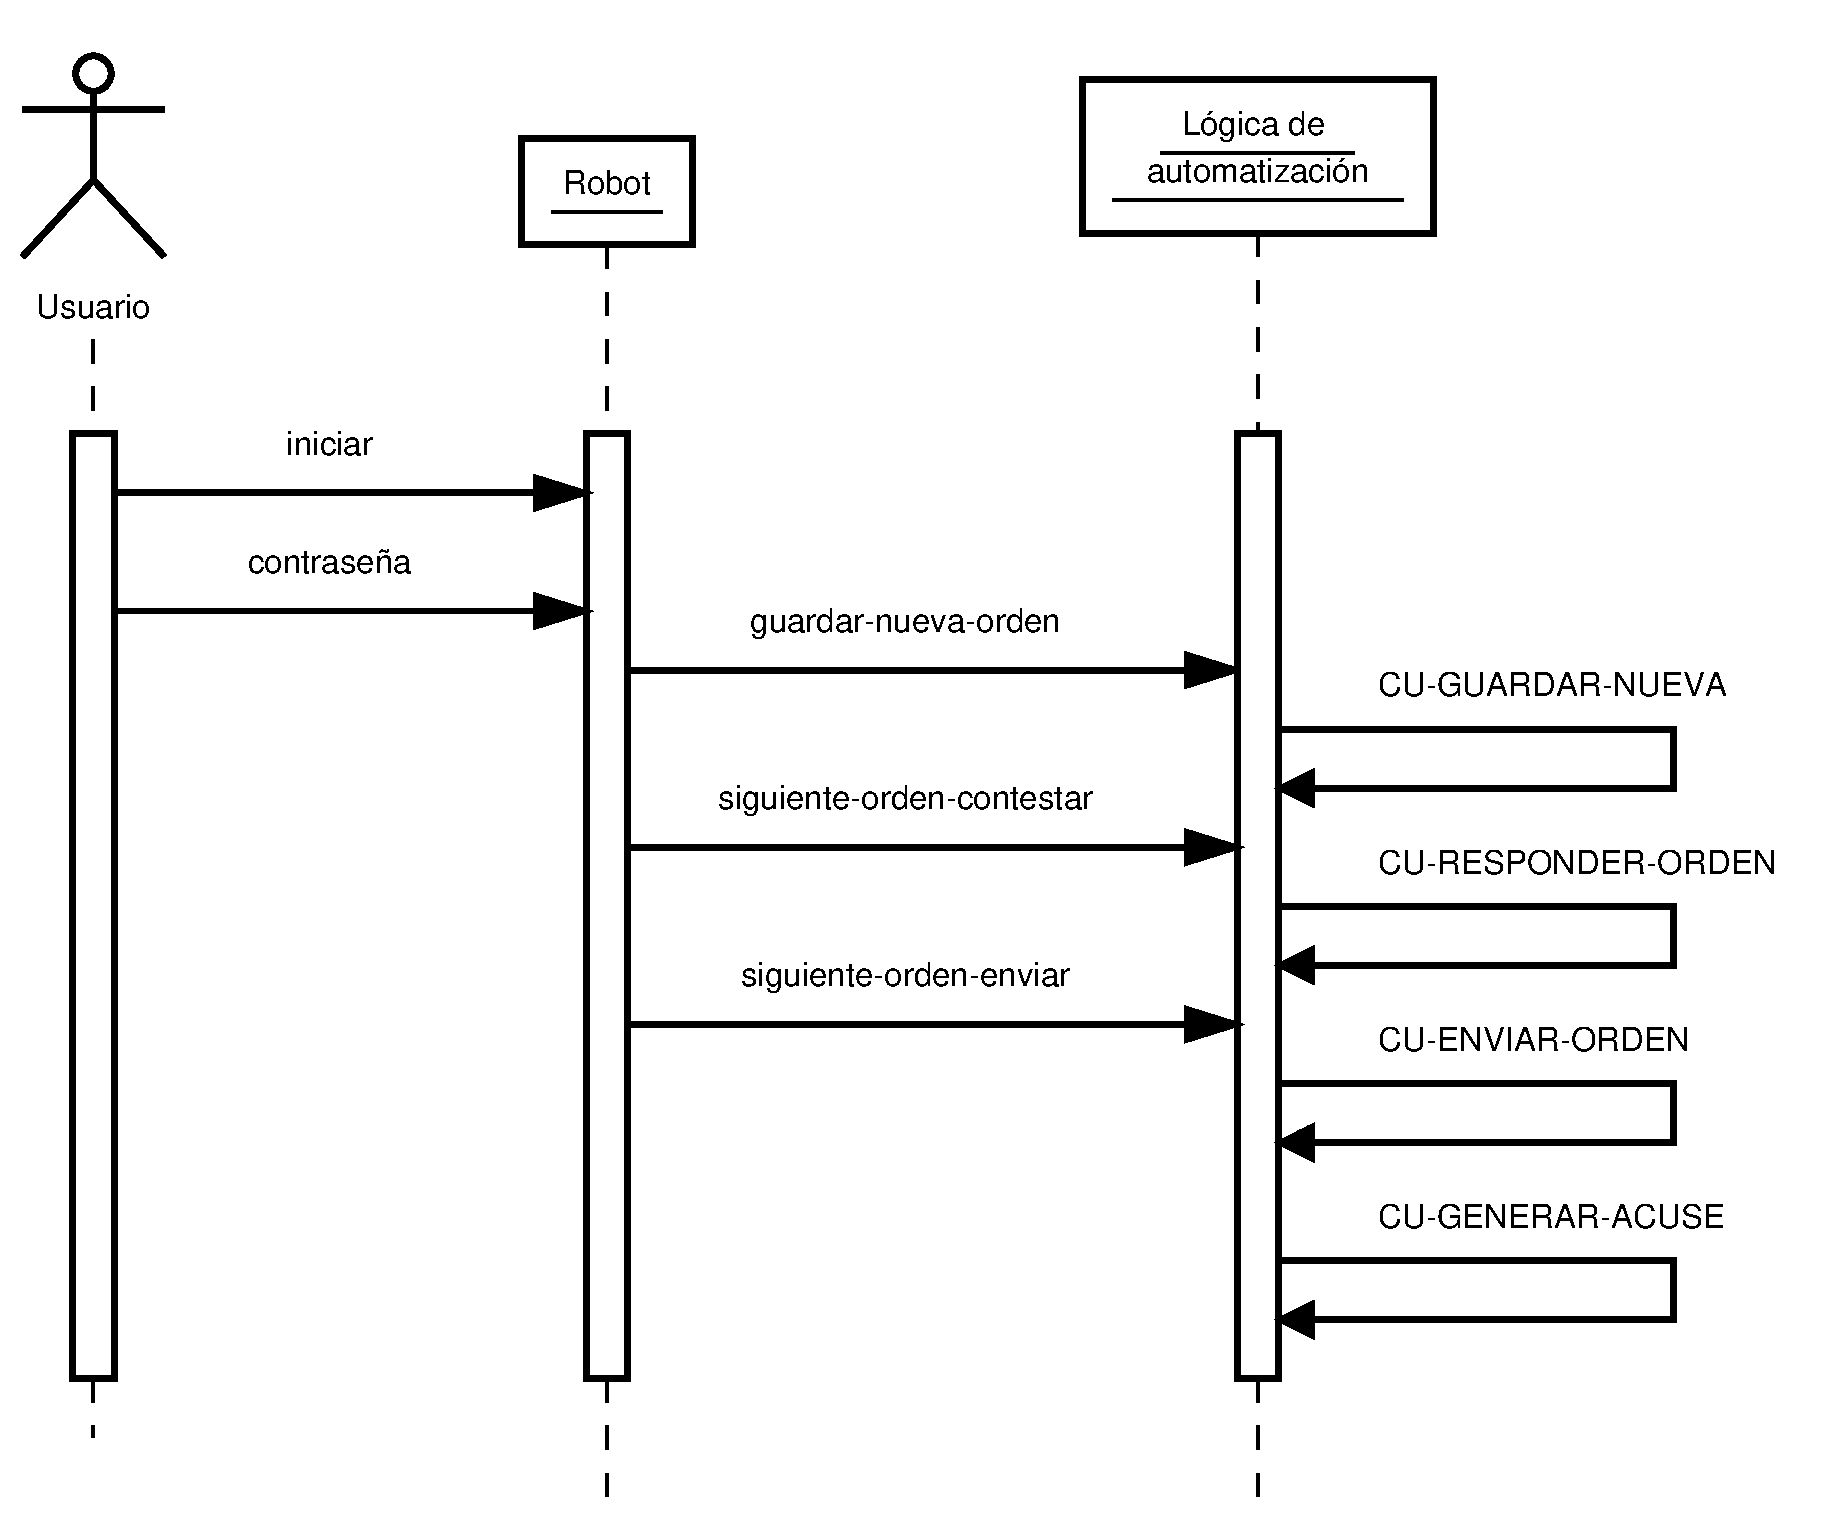
\includegraphics[width=\textwidth]{dia-seq-cu-contestar}
	\caption{Diagrama de secuencia caso de uso contestar órdenes.}
	\label{fig:dia-seq-cu-contestar}
\end{figure}
\subsubsection{Generar acuse de envío}
Ver sección \ref{cu-contestar}.\\
\begin{figure}[h]
	\centering
	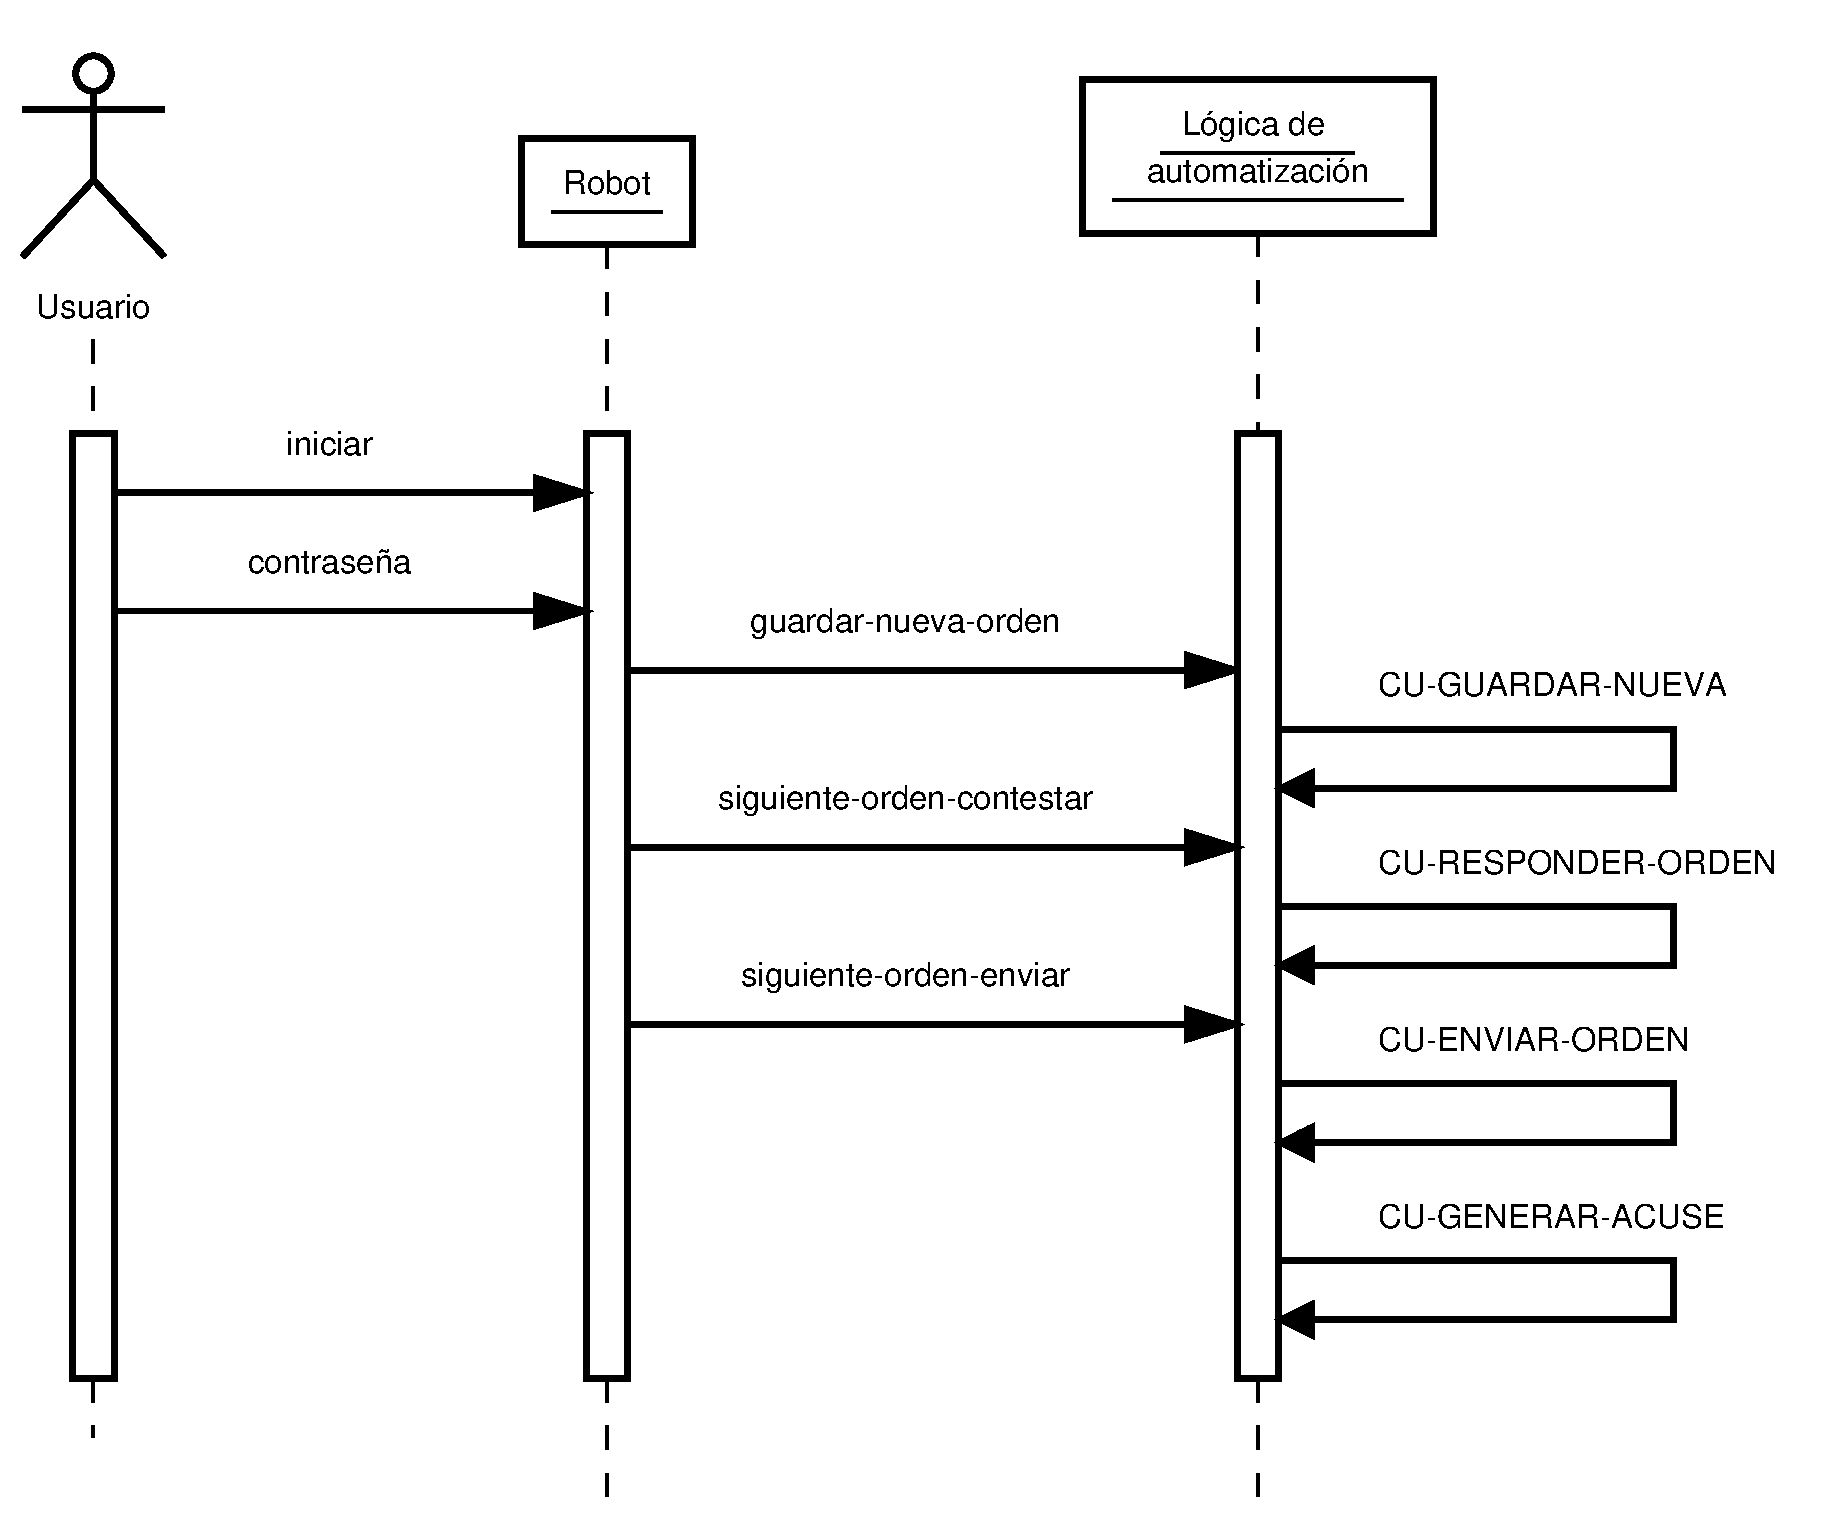
\includegraphics[width=\textwidth]{dia-seq-cu-contestar}
	\caption{Diagrama de secuencia caso de uso contestar órdenes.}
	\label{fig:dia-seq-cu-contestar}
\end{figure}
\subsubsection{Verificar órdenes}
Ver sección \ref{cu-contestar}.\\
\begin{figure}[h]
	\centering
	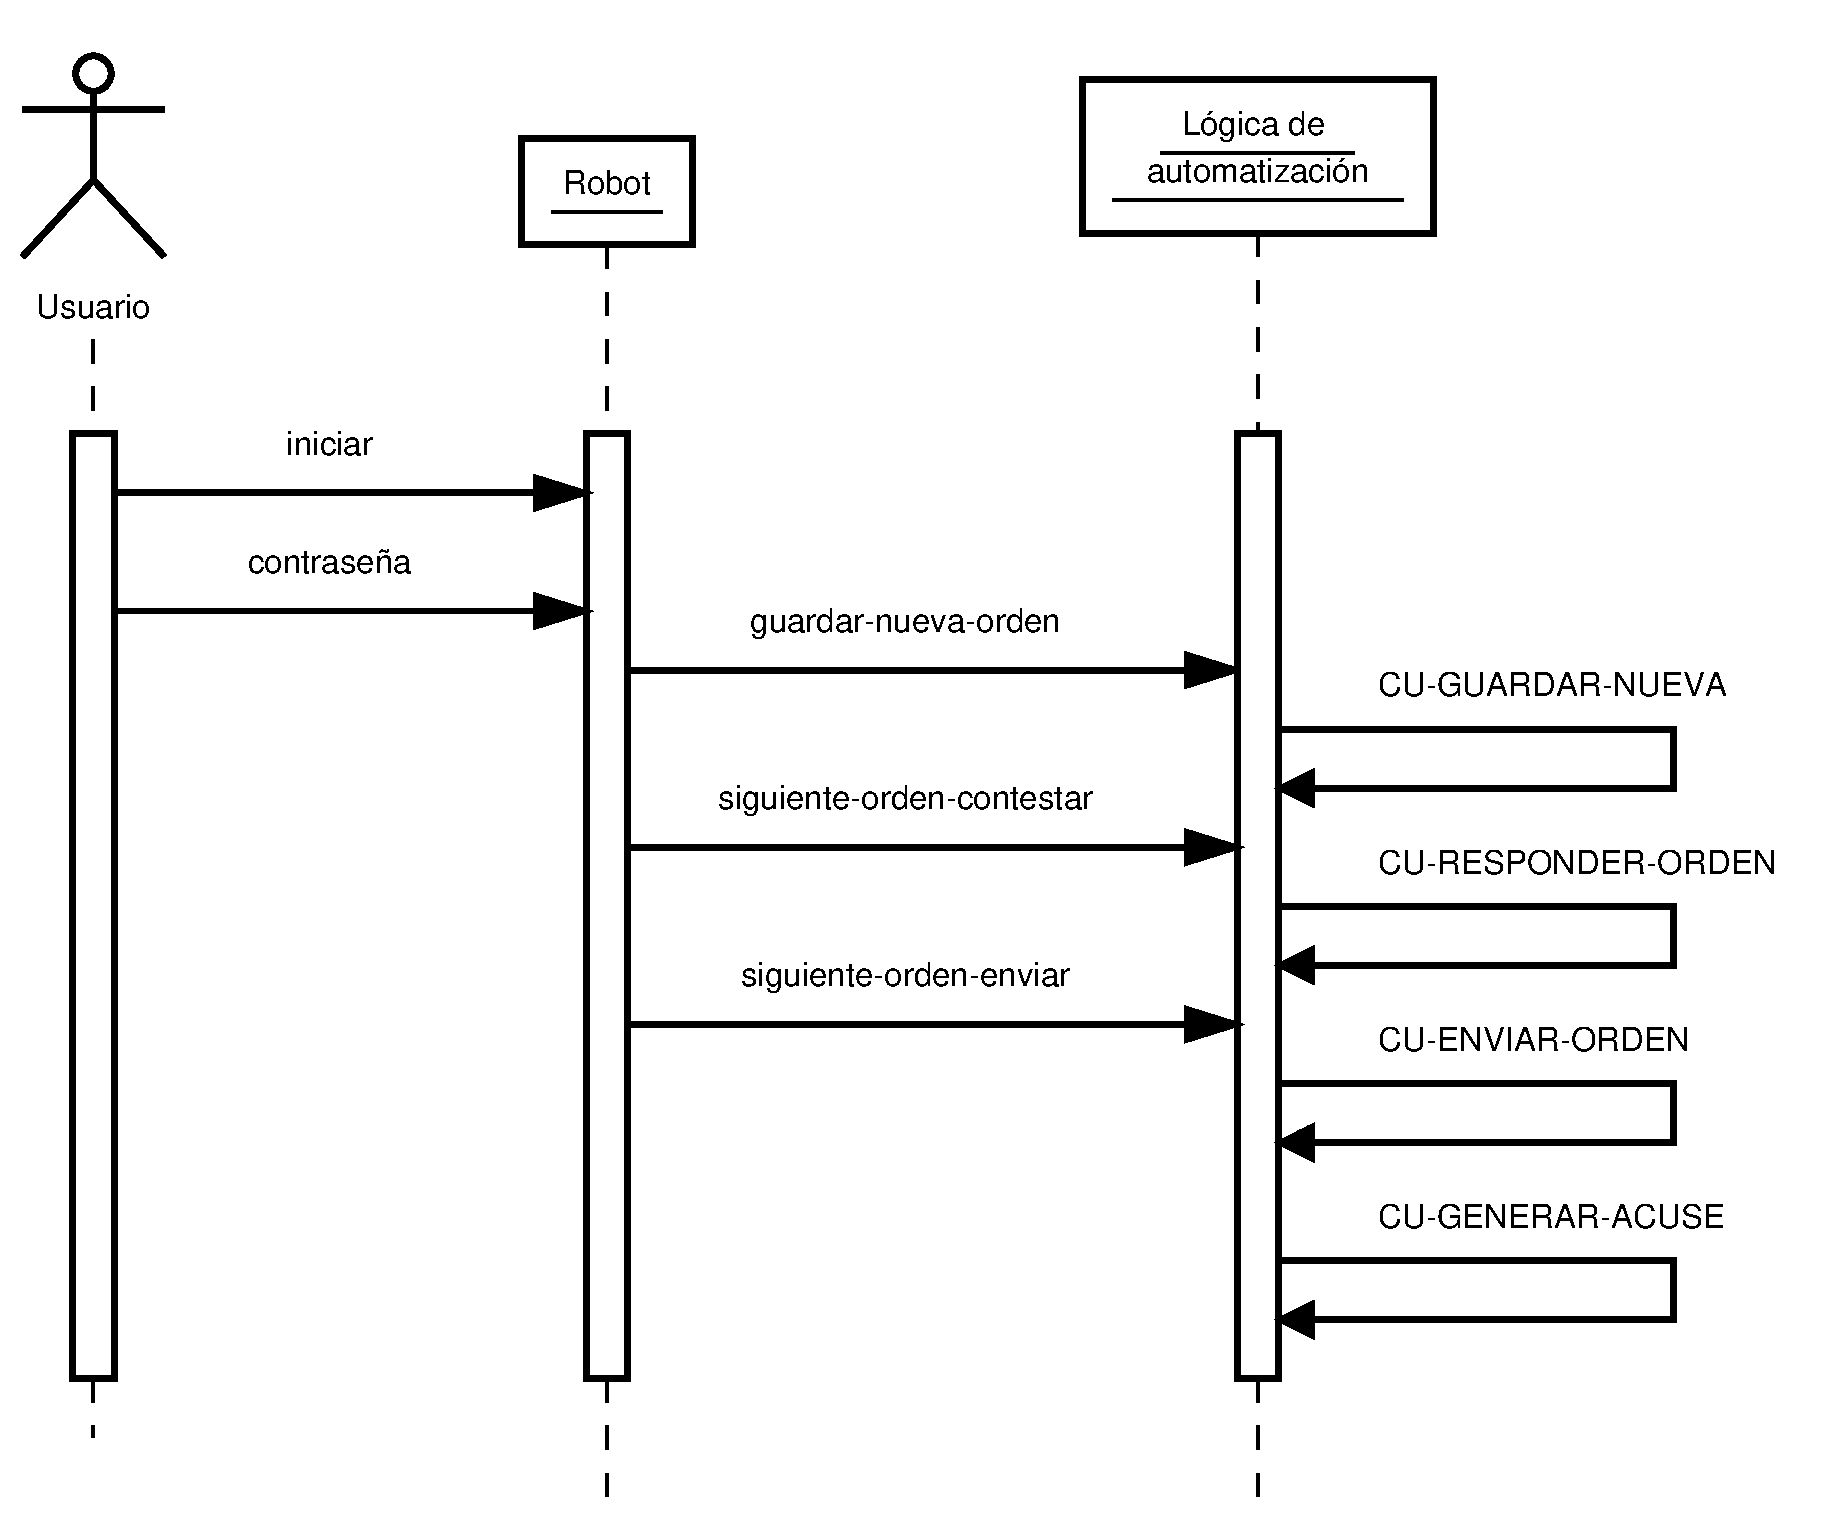
\includegraphics[width=\textwidth]{dia-seq-cu-contestar}
	\caption{Diagrama de secuencia caso de uso contestar órdenes.}
	\label{fig:dia-seq-cu-contestar}
\end{figure}
\subsubsection{Actualizar estatus SA}
Ver sección \ref{cu-contestar}.\\
\begin{figure}[h]
	\centering
	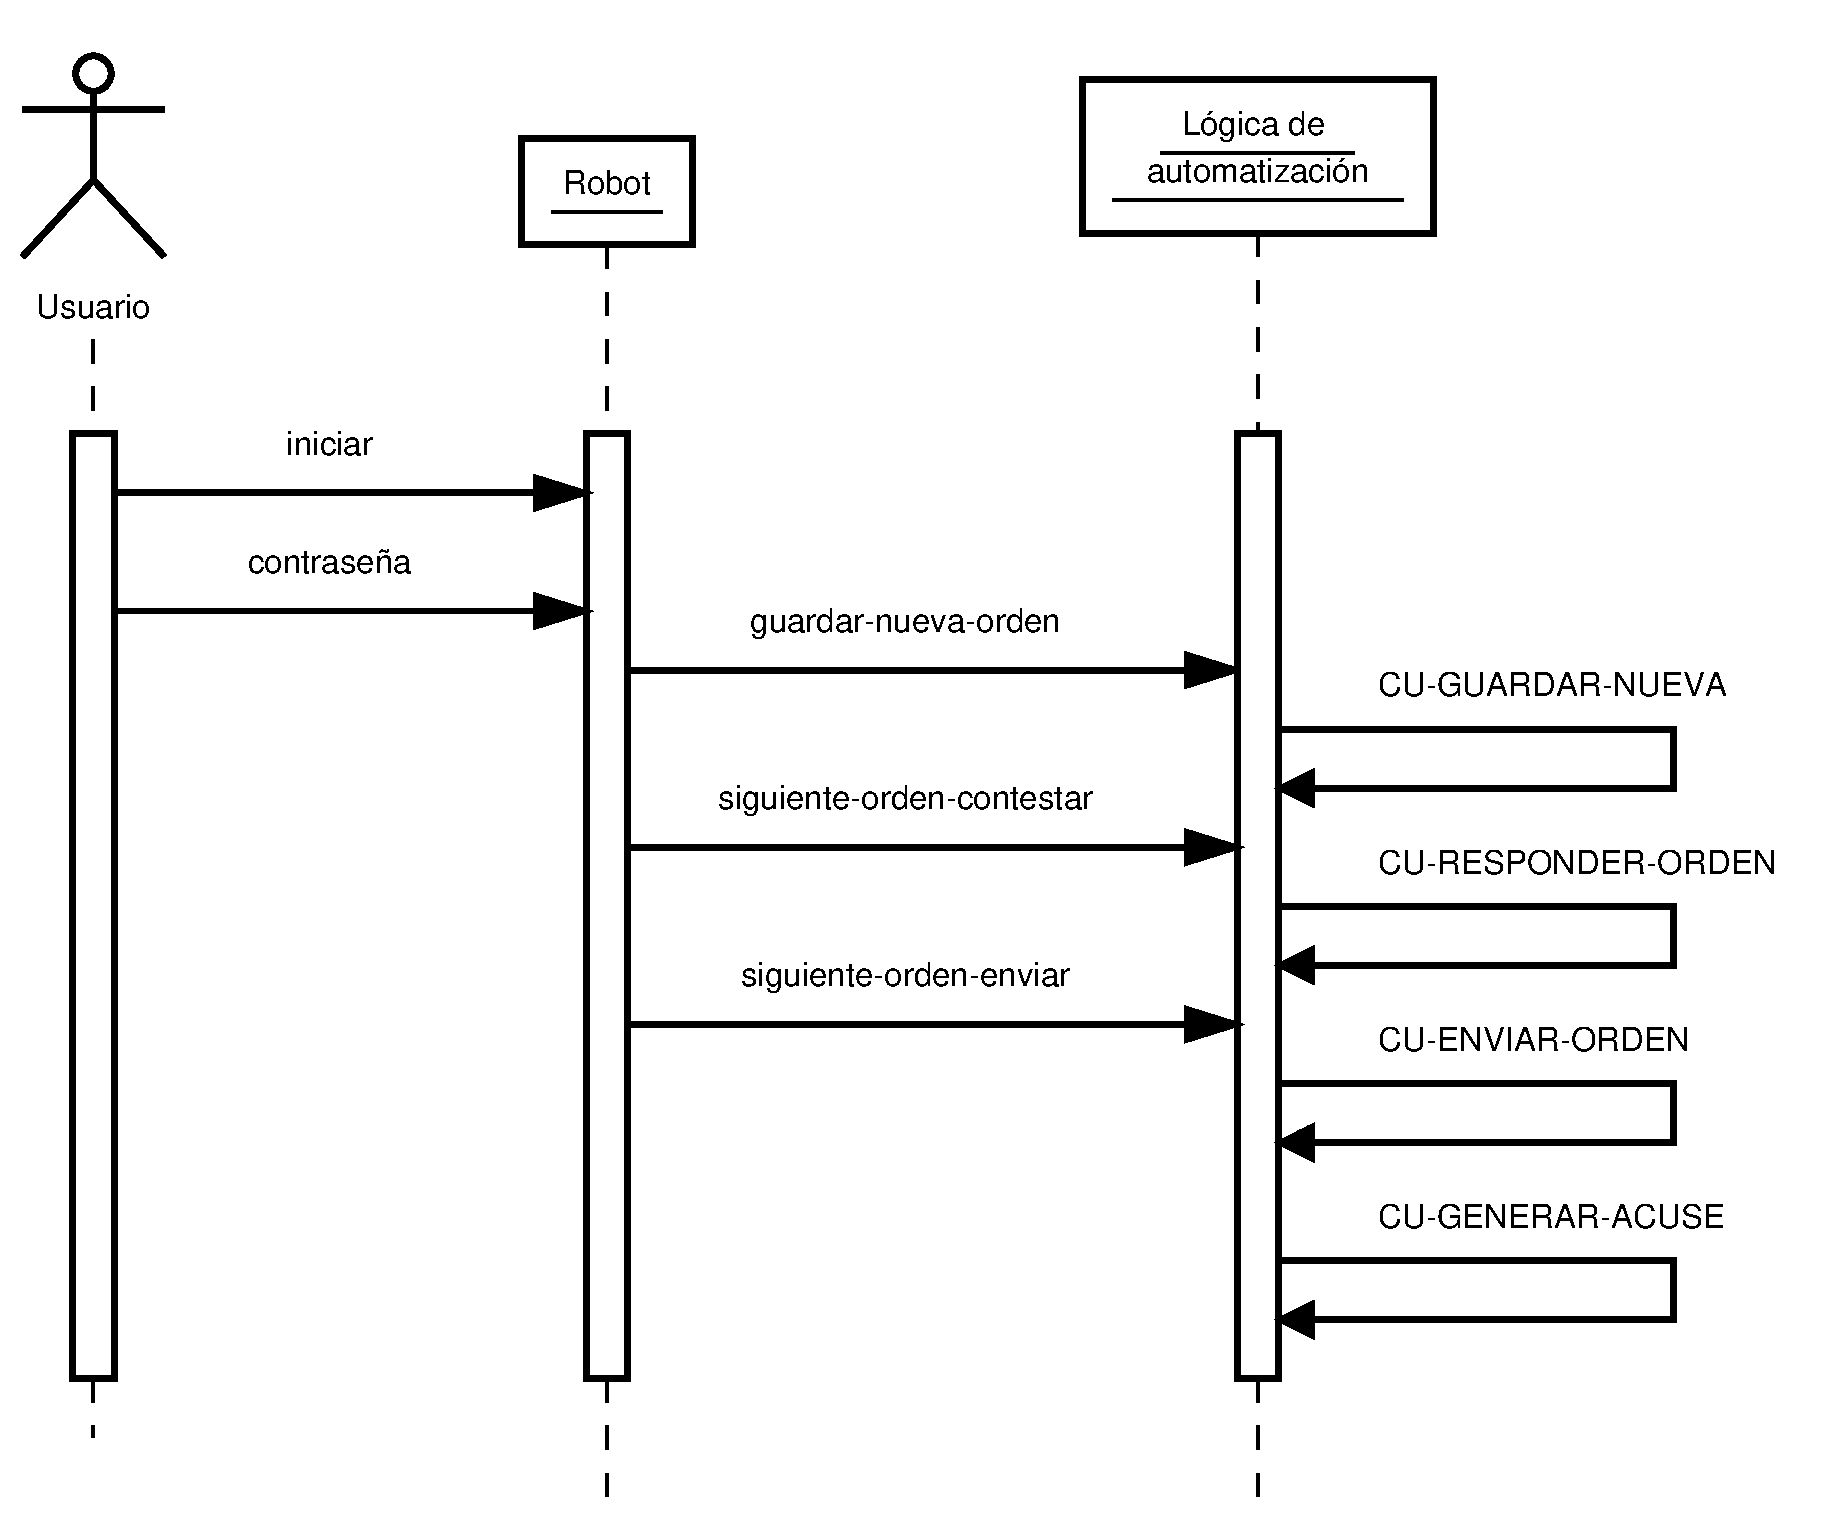
\includegraphics[width=\textwidth]{dia-seq-cu-contestar}
	\caption{Diagrama de secuencia caso de uso contestar órdenes.}
	\label{fig:dia-seq-cu-contestar}
\end{figure}
\subsubsection{Entrar en interfaz Web}
Ver sección \ref{cu-contestar}.\\
\begin{figure}[h]
	\centering
	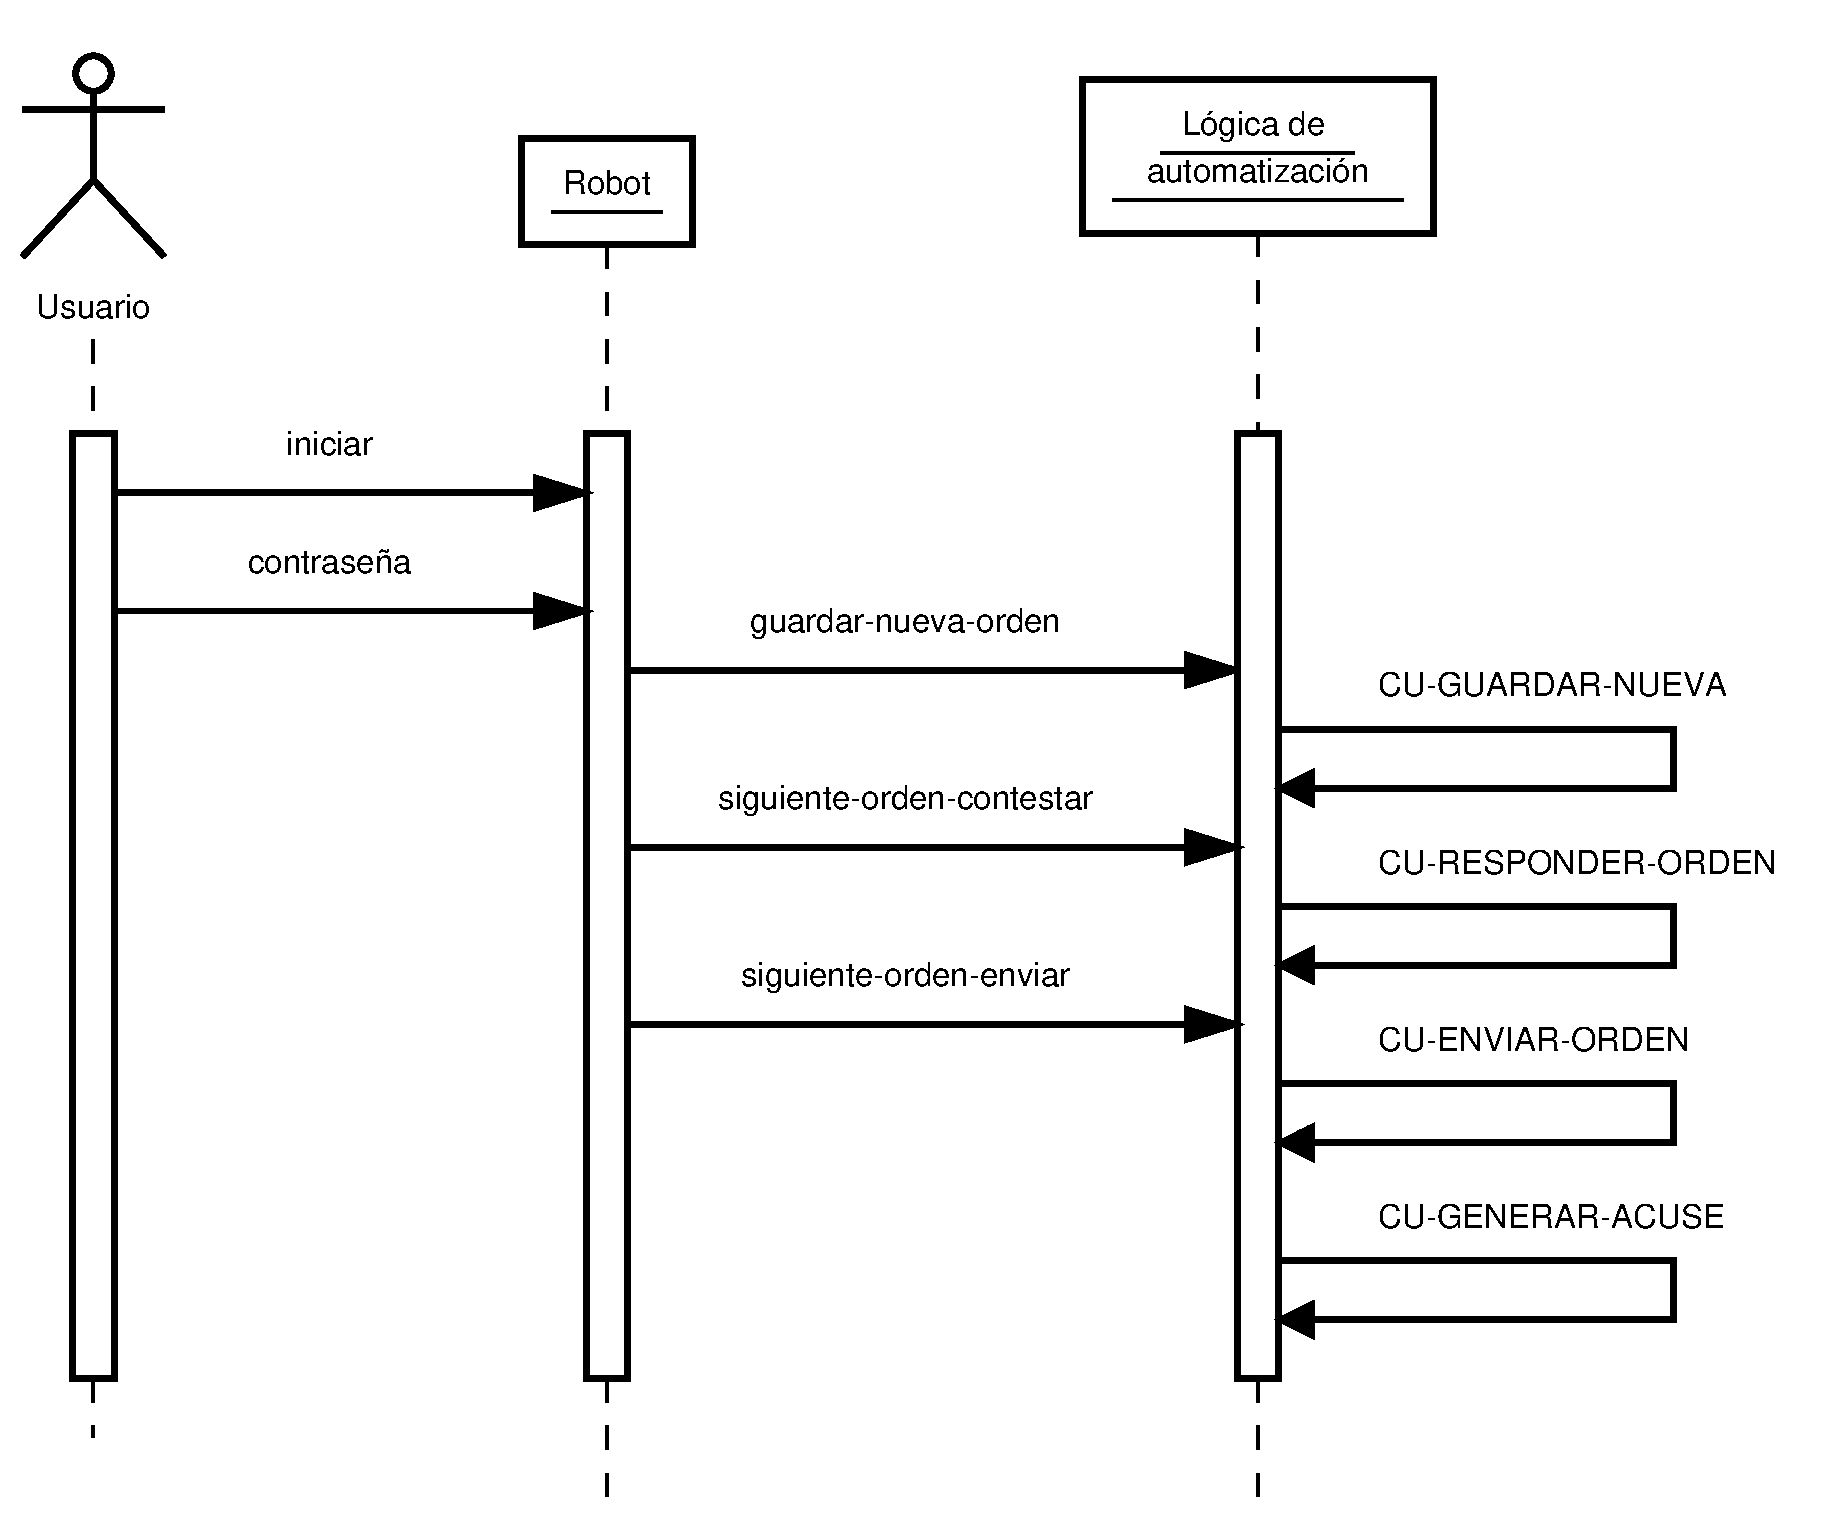
\includegraphics[width=\textwidth]{dia-seq-cu-contestar}
	\caption{Diagrama de secuencia caso de uso contestar órdenes.}
	\label{fig:dia-seq-cu-contestar}
\end{figure}
\subsubsection{Generar reporte}
Ver sección \ref{cu-contestar}.\\
\begin{figure}[h]
	\centering
	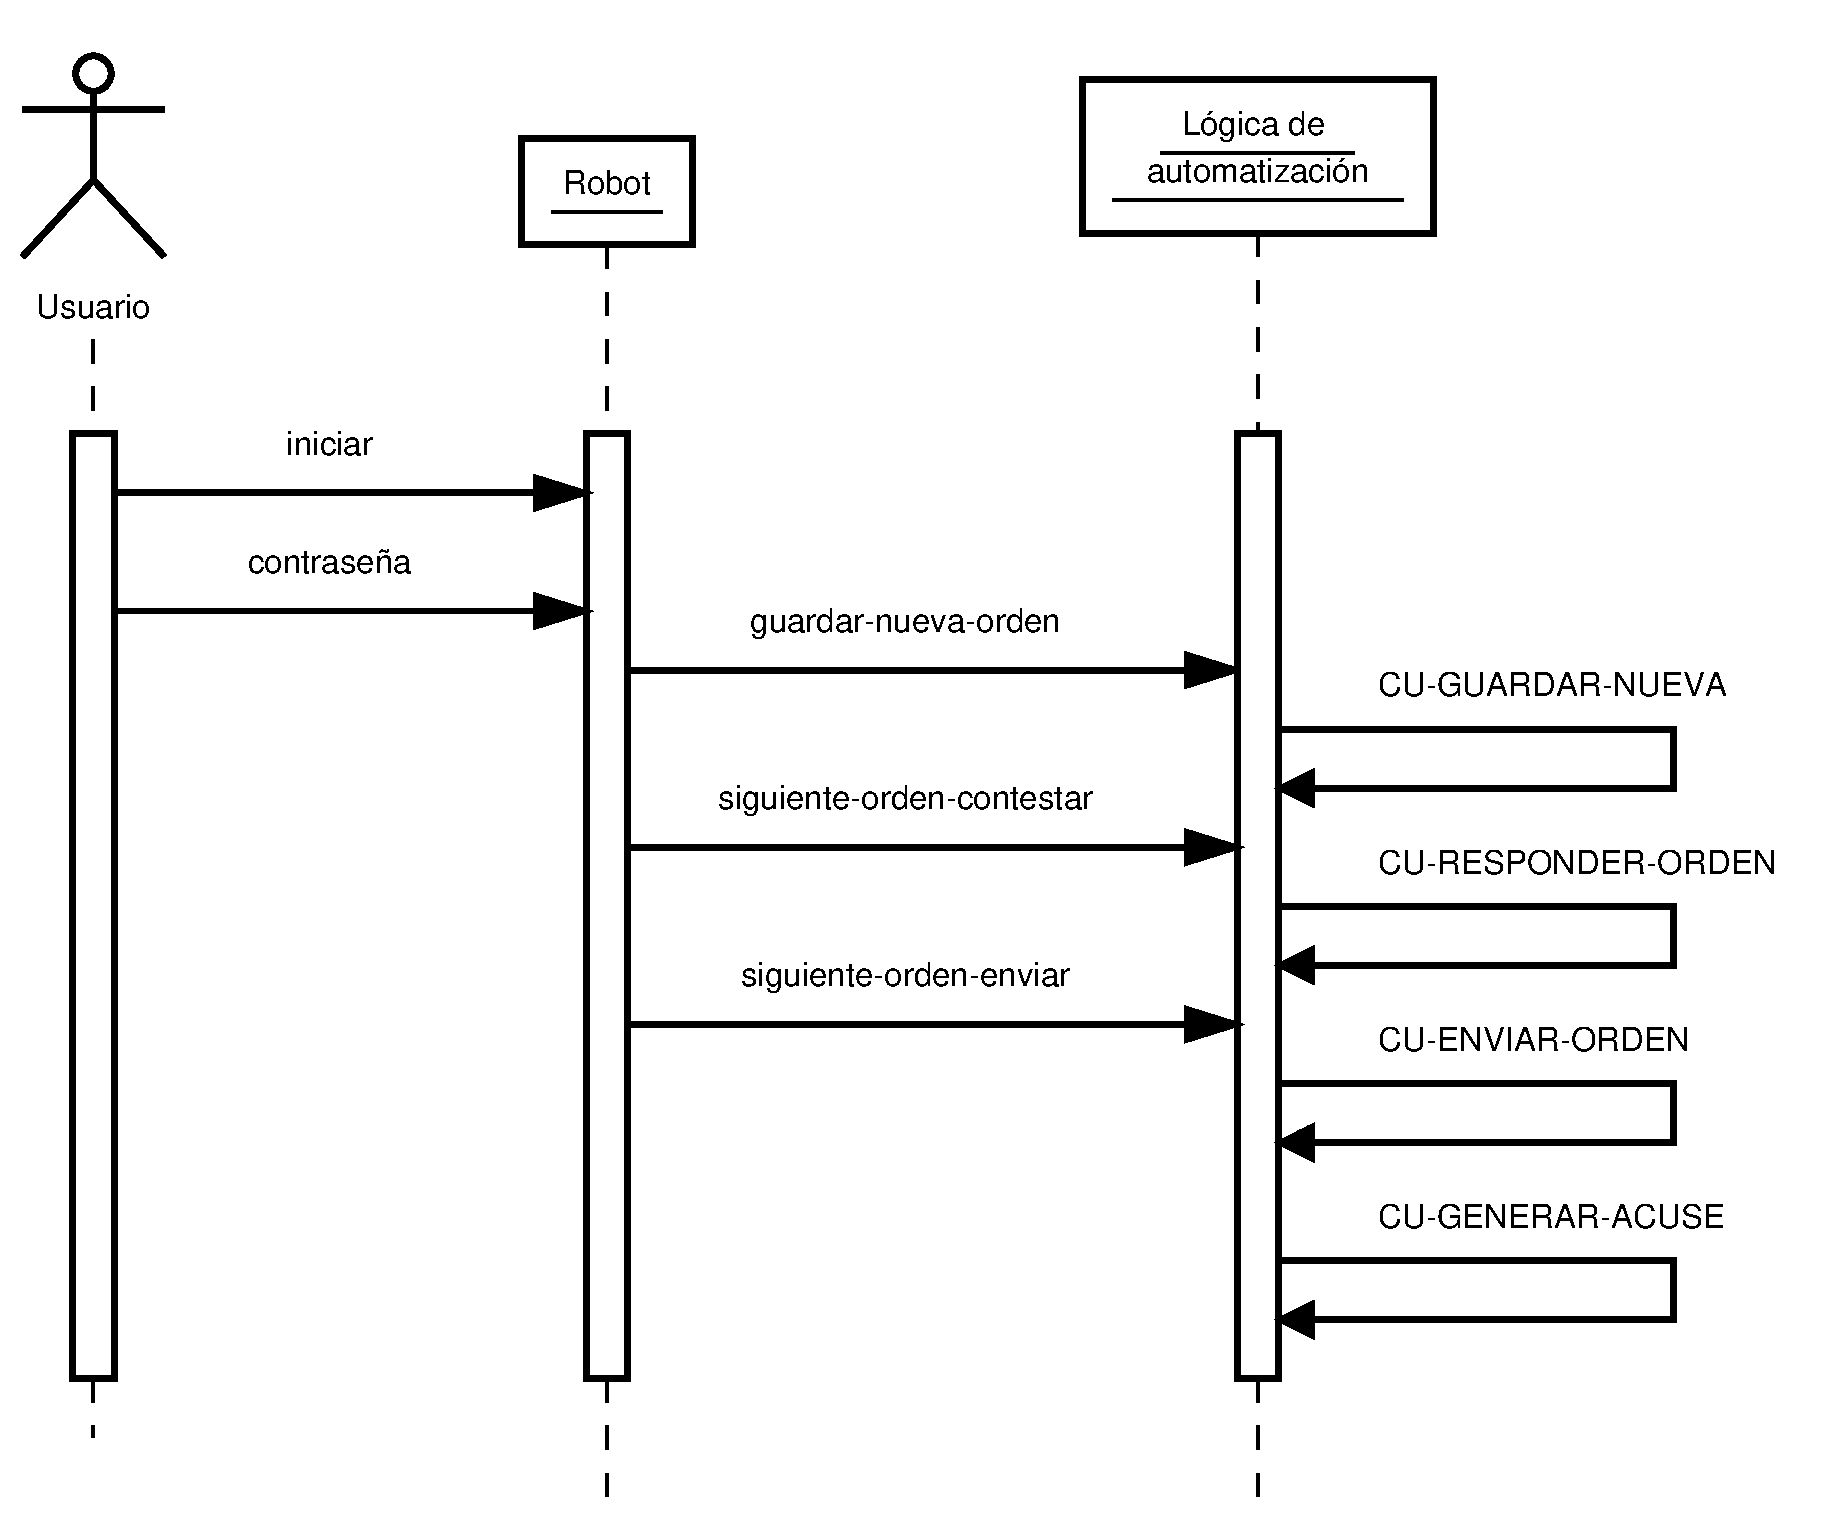
\includegraphics[width=\textwidth]{dia-seq-cu-contestar}
	\caption{Diagrama de secuencia caso de uso contestar órdenes.}
	\label{fig:dia-seq-cu-contestar}
\end{figure}
\subsubsection{Actualizar catálogo}
Ver sección \ref{cu-contestar}.\\
\begin{figure}[h]
	\centering
	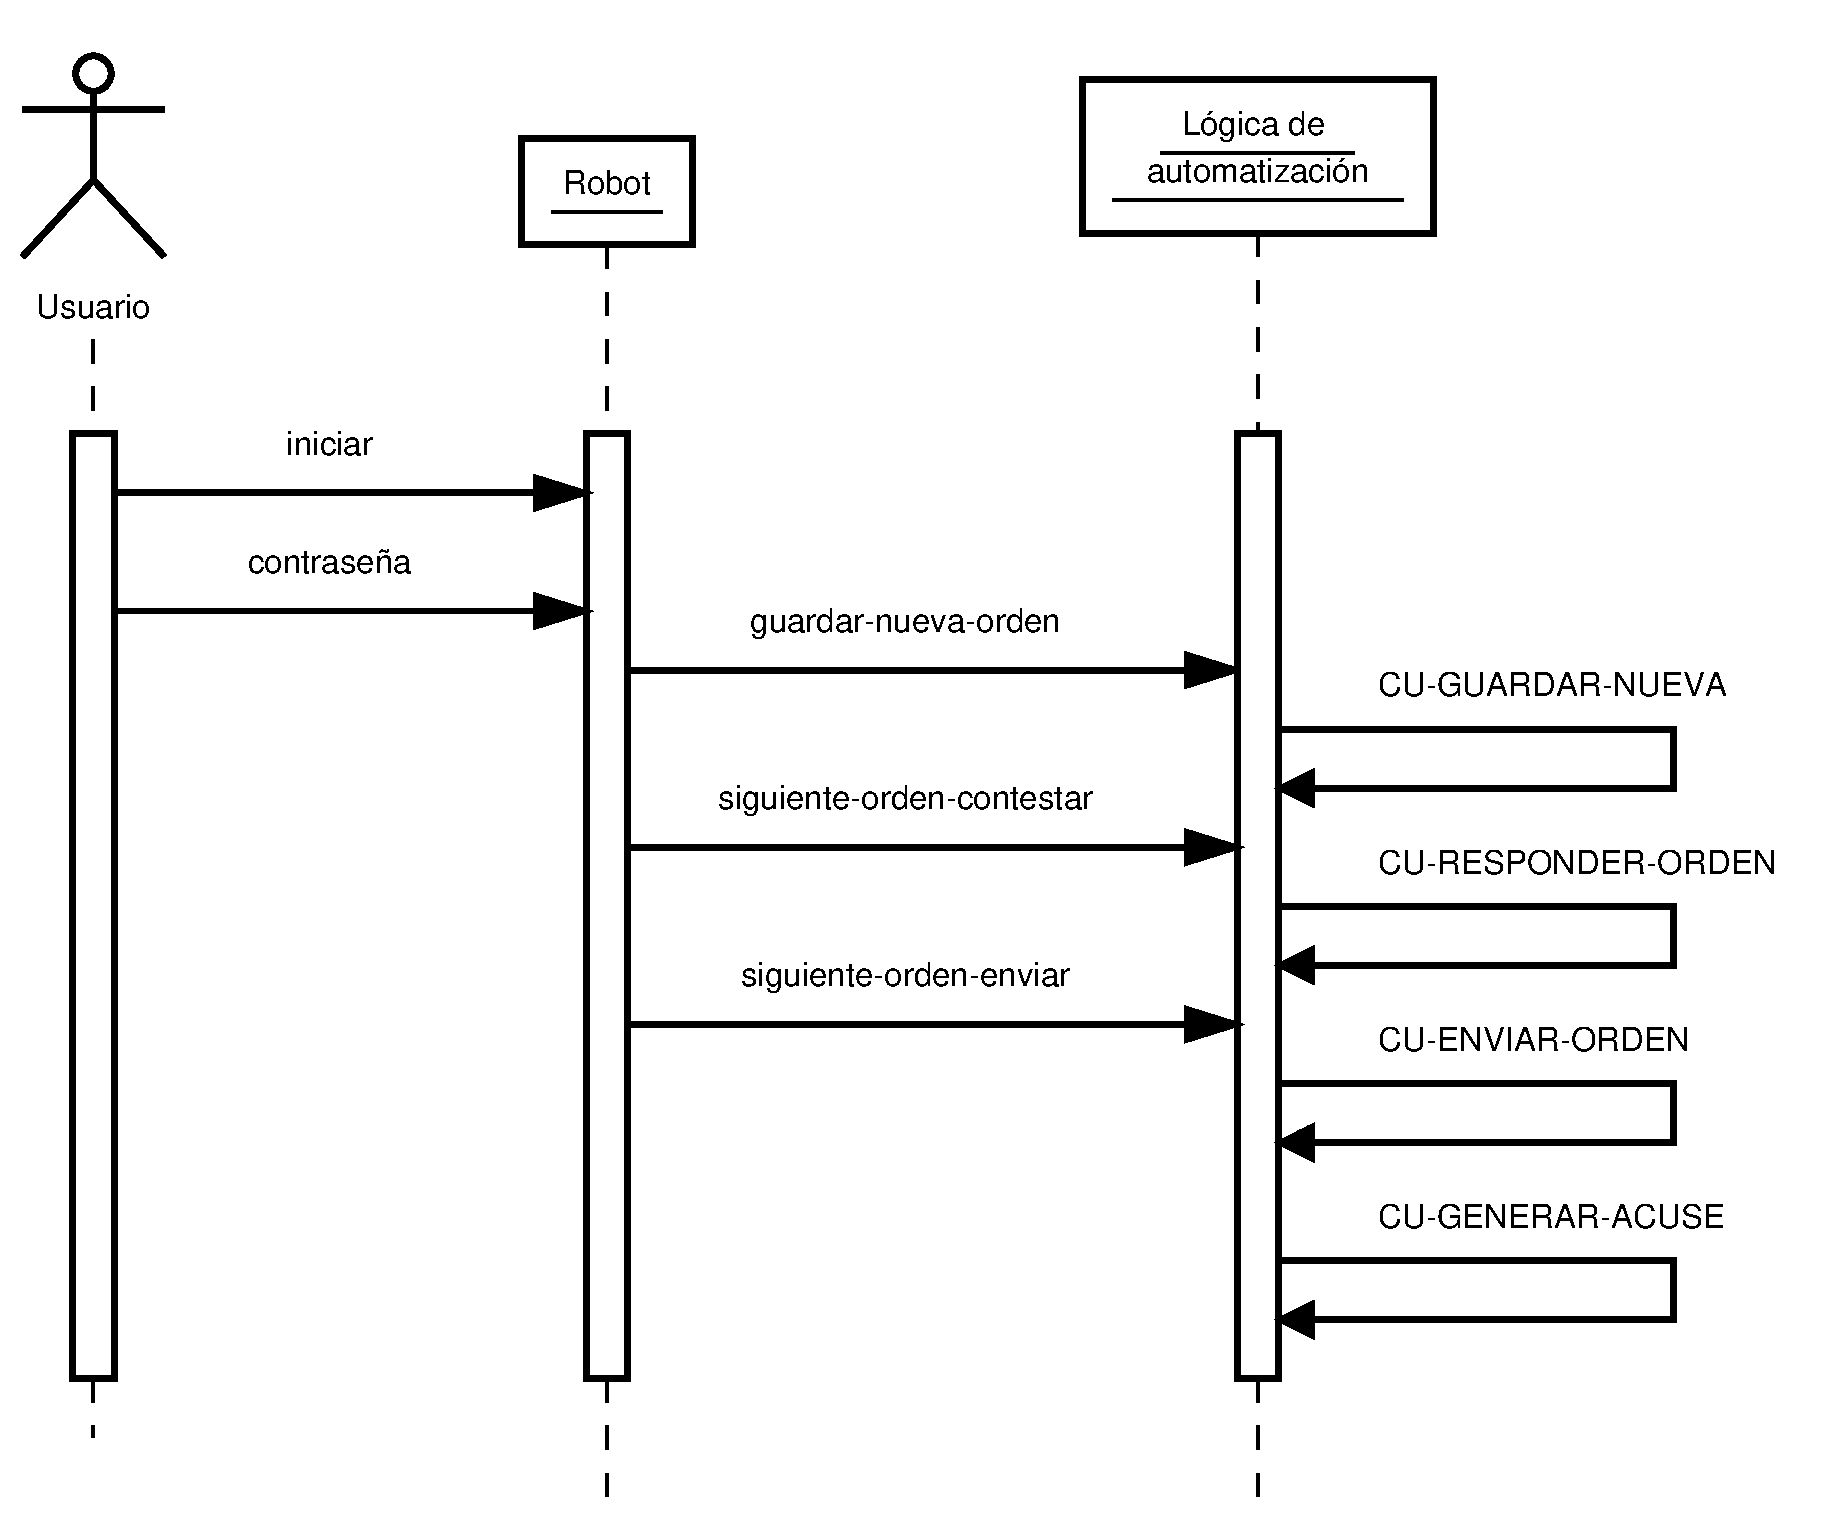
\includegraphics[width=\textwidth]{dia-seq-cu-contestar}
	\caption{Diagrama de secuencia caso de uso contestar órdenes.}
	\label{fig:dia-seq-cu-contestar}
\end{figure}
\subsubsection{Buscar órdenes}
Ver sección \ref{cu-contestar}.\\
\begin{figure}[h]
	\centering
	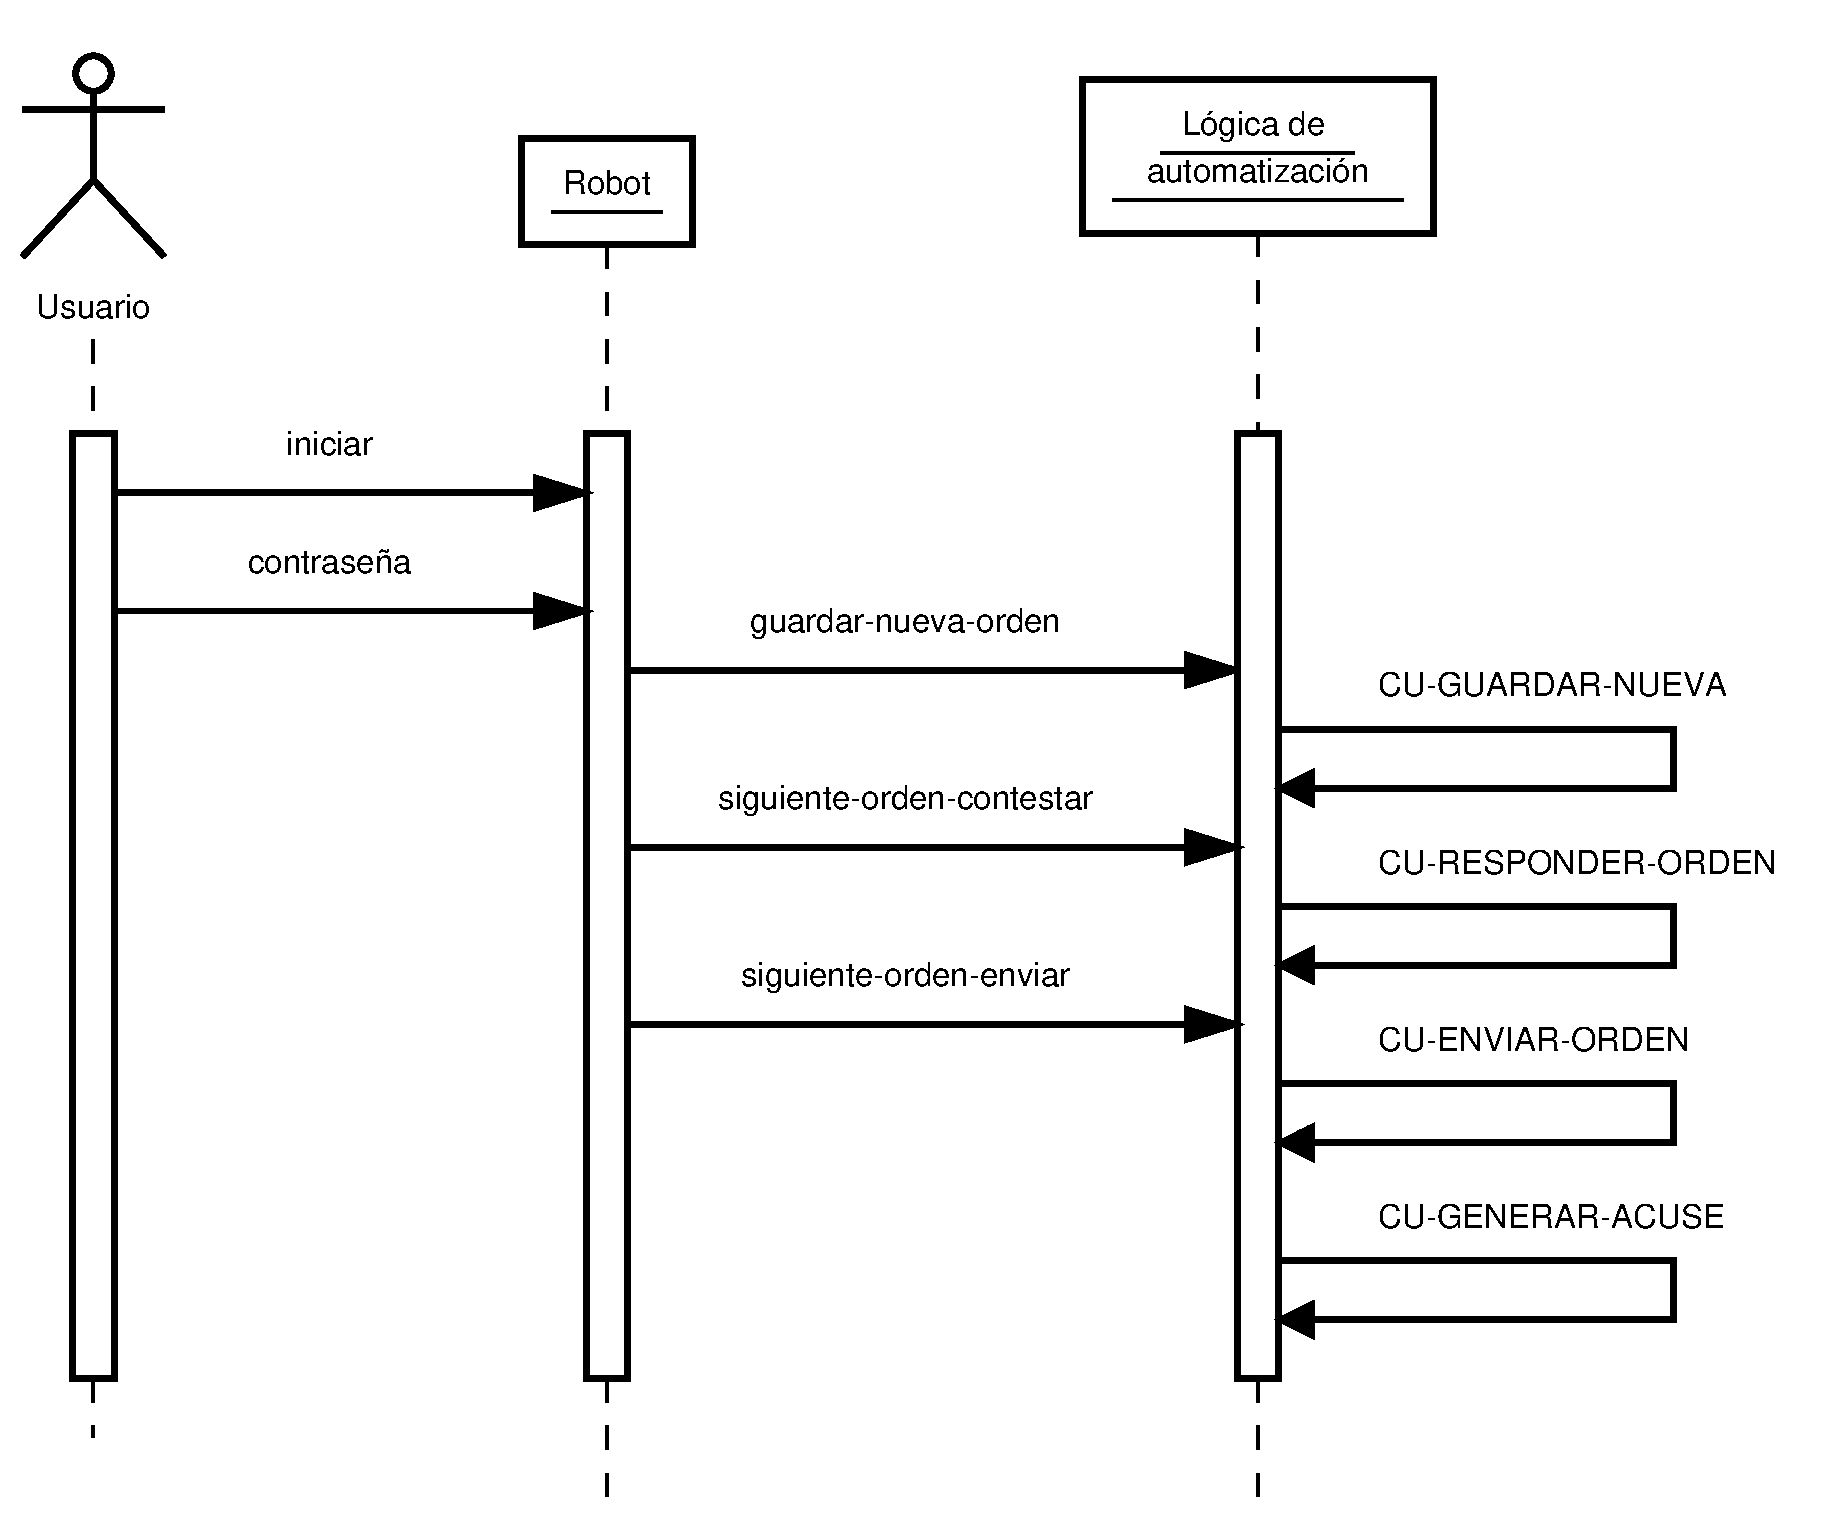
\includegraphics[width=\textwidth]{dia-seq-cu-contestar}
	\caption{Diagrama de secuencia caso de uso contestar órdenes.}
	\label{fig:dia-seq-cu-contestar}
\end{figure}
\subsubsection{Visualizar orden}
Ver sección \ref{cu-contestar}.\\
\begin{figure}[h]
	\centering
	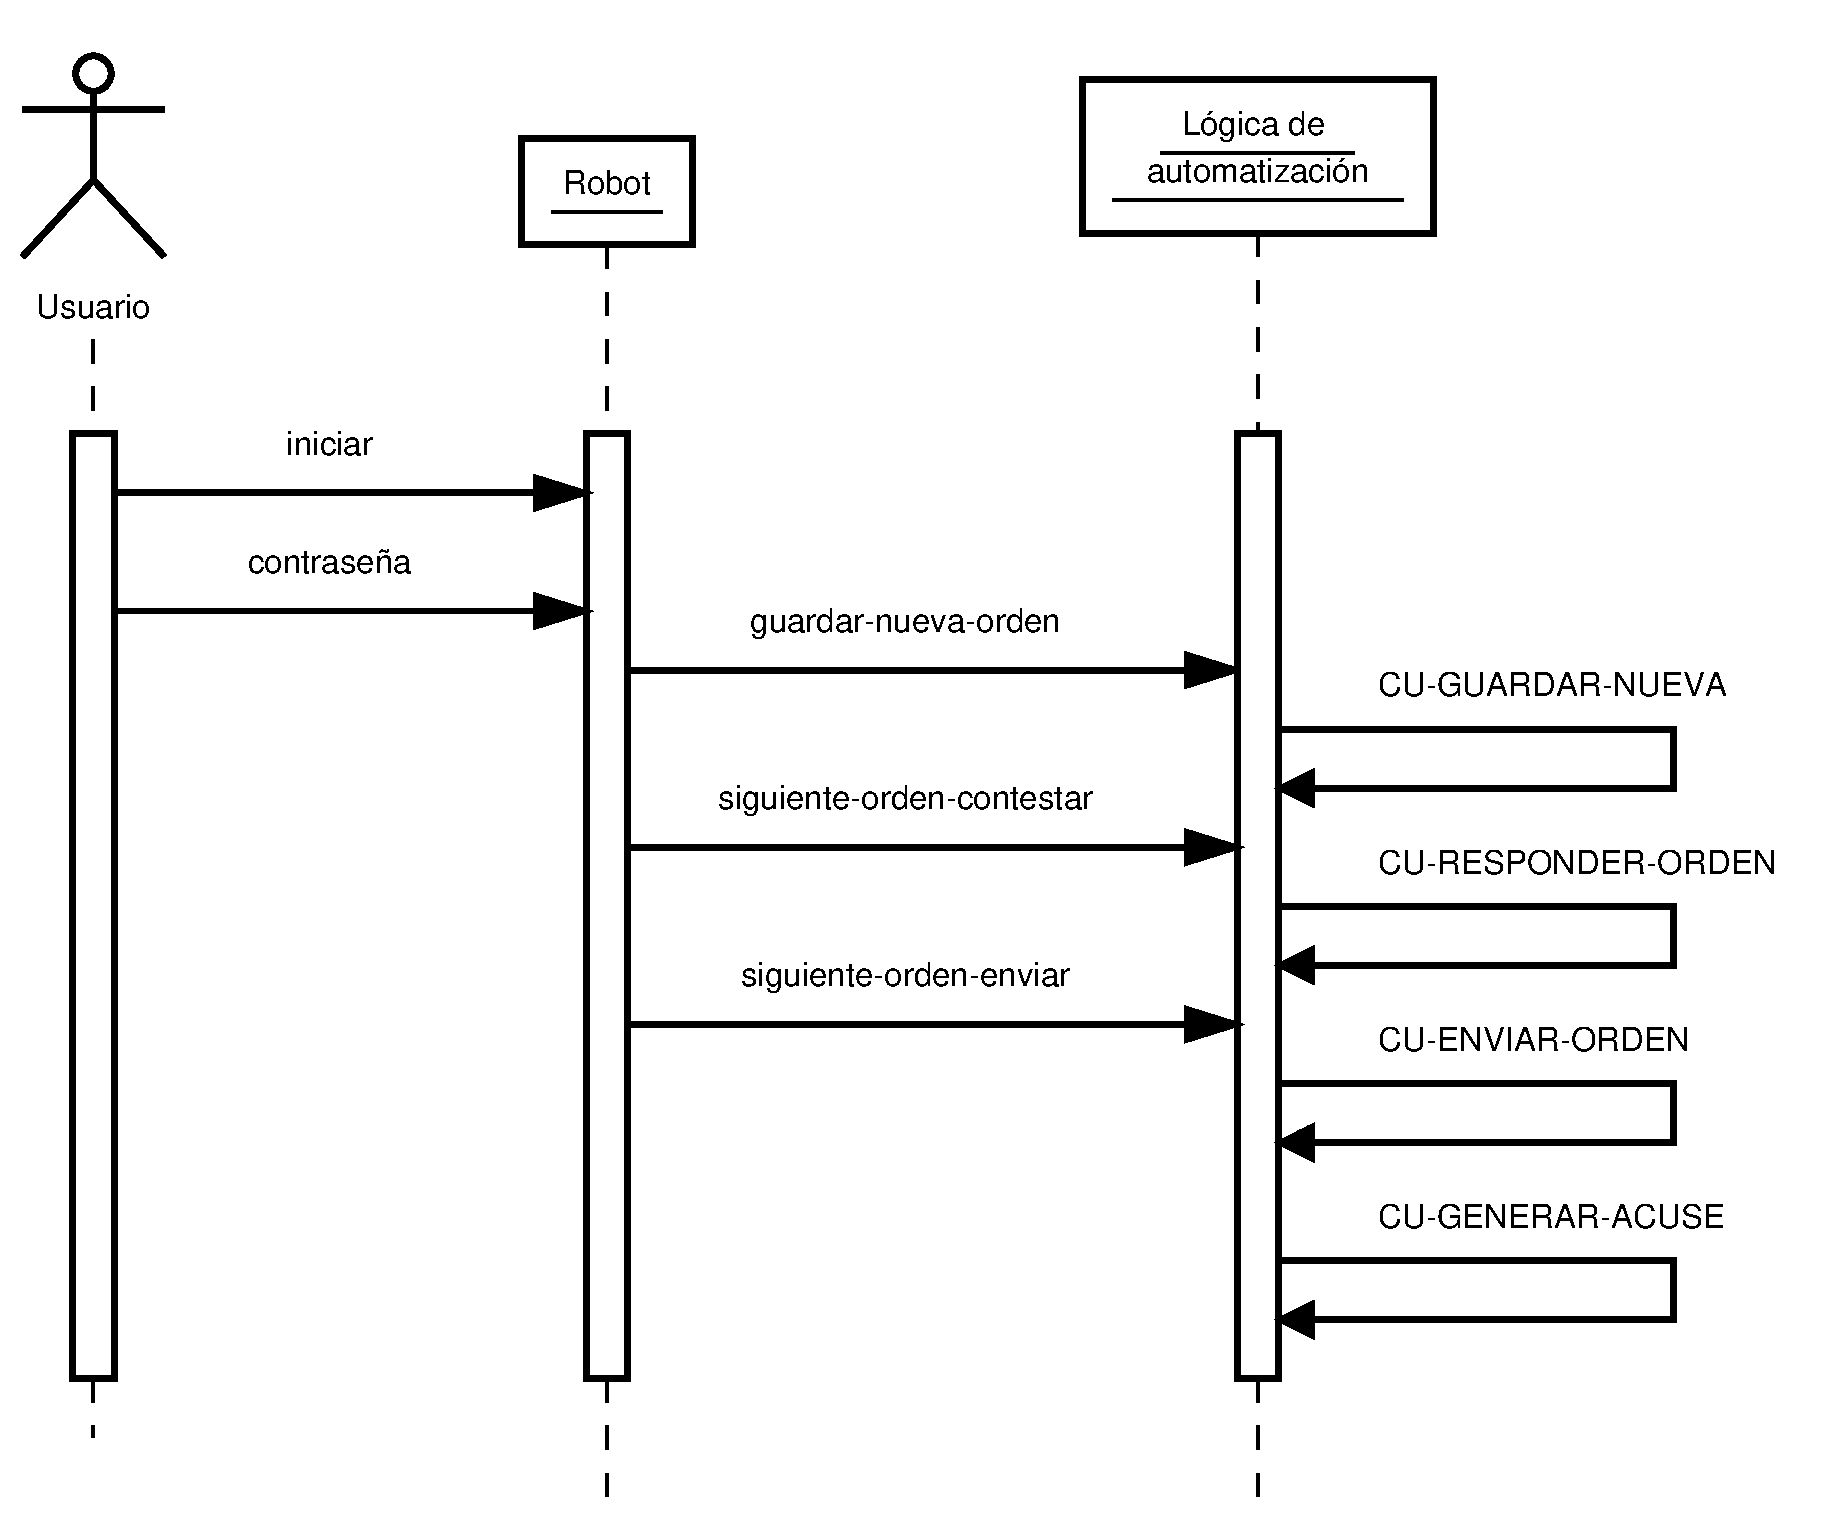
\includegraphics[width=\textwidth]{dia-seq-cu-contestar}
	\caption{Diagrama de secuencia caso de uso contestar órdenes.}
	\label{fig:dia-seq-cu-contestar}
\end{figure}
\subsubsection{Editar orden}
Ver sección \ref{cu-contestar}.\\
\begin{figure}[h]
	\centering
	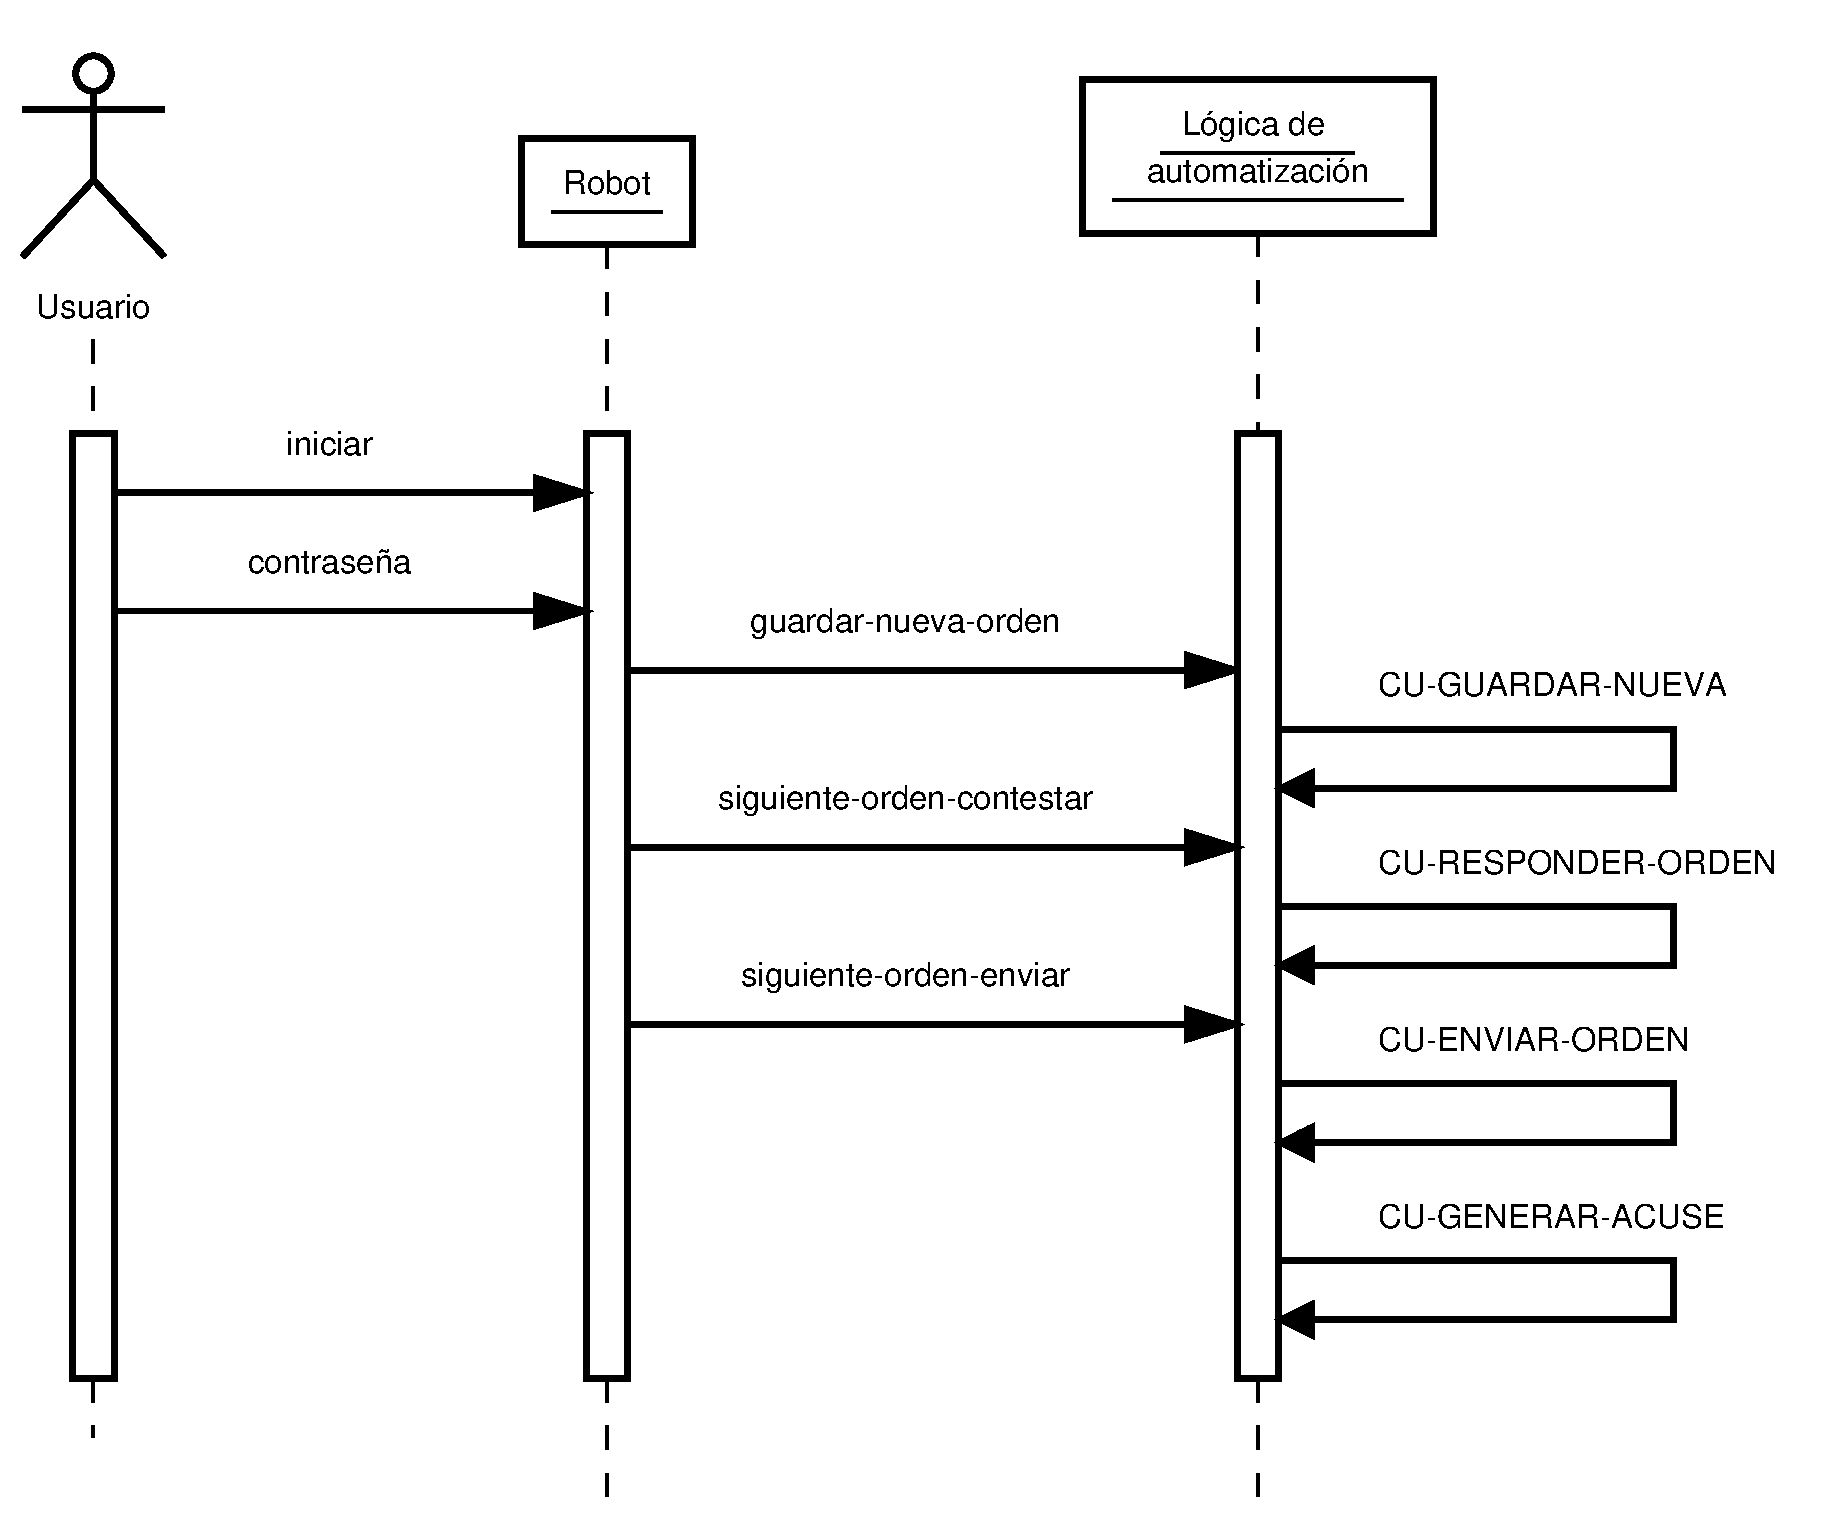
\includegraphics[width=\textwidth]{dia-seq-cu-contestar}
	\caption{Diagrama de secuencia caso de uso contestar órdenes.}
	\label{fig:dia-seq-cu-contestar}
\end{figure}
\fi


%===============================================================================
%===============================================================================


\section{Diseño de la base de datos}
La base de datos tiene dos finalidades, guardar la información capturada de las órdenes de reposición atendidas así como los catálogos necesarios para los procesos automatizados y generación de reportes; la segunda es guardar la información de los usuarios autorizados para utilizar el portal web.\\
El diseño de la base de datos se centra en los siguientes grupos\footnote{Los nombres de las tablas están escritos utilizando letras minúsculas de alfabeto inglés y guión bajo $([a-z]{\textunderscore})^+$}(ver Figura \ref{fig:dia-er-resumen}):
\begin{enumerate}
	\item Tablas del registro de eventos.
	\item Tablas de las órdenes de reposición.
	\item Tablas de los usuarios de la interfaz web.
	\item Catálogos para generación de reportes.
\end{enumerate}
\begin{figure}[h]
  \centering
  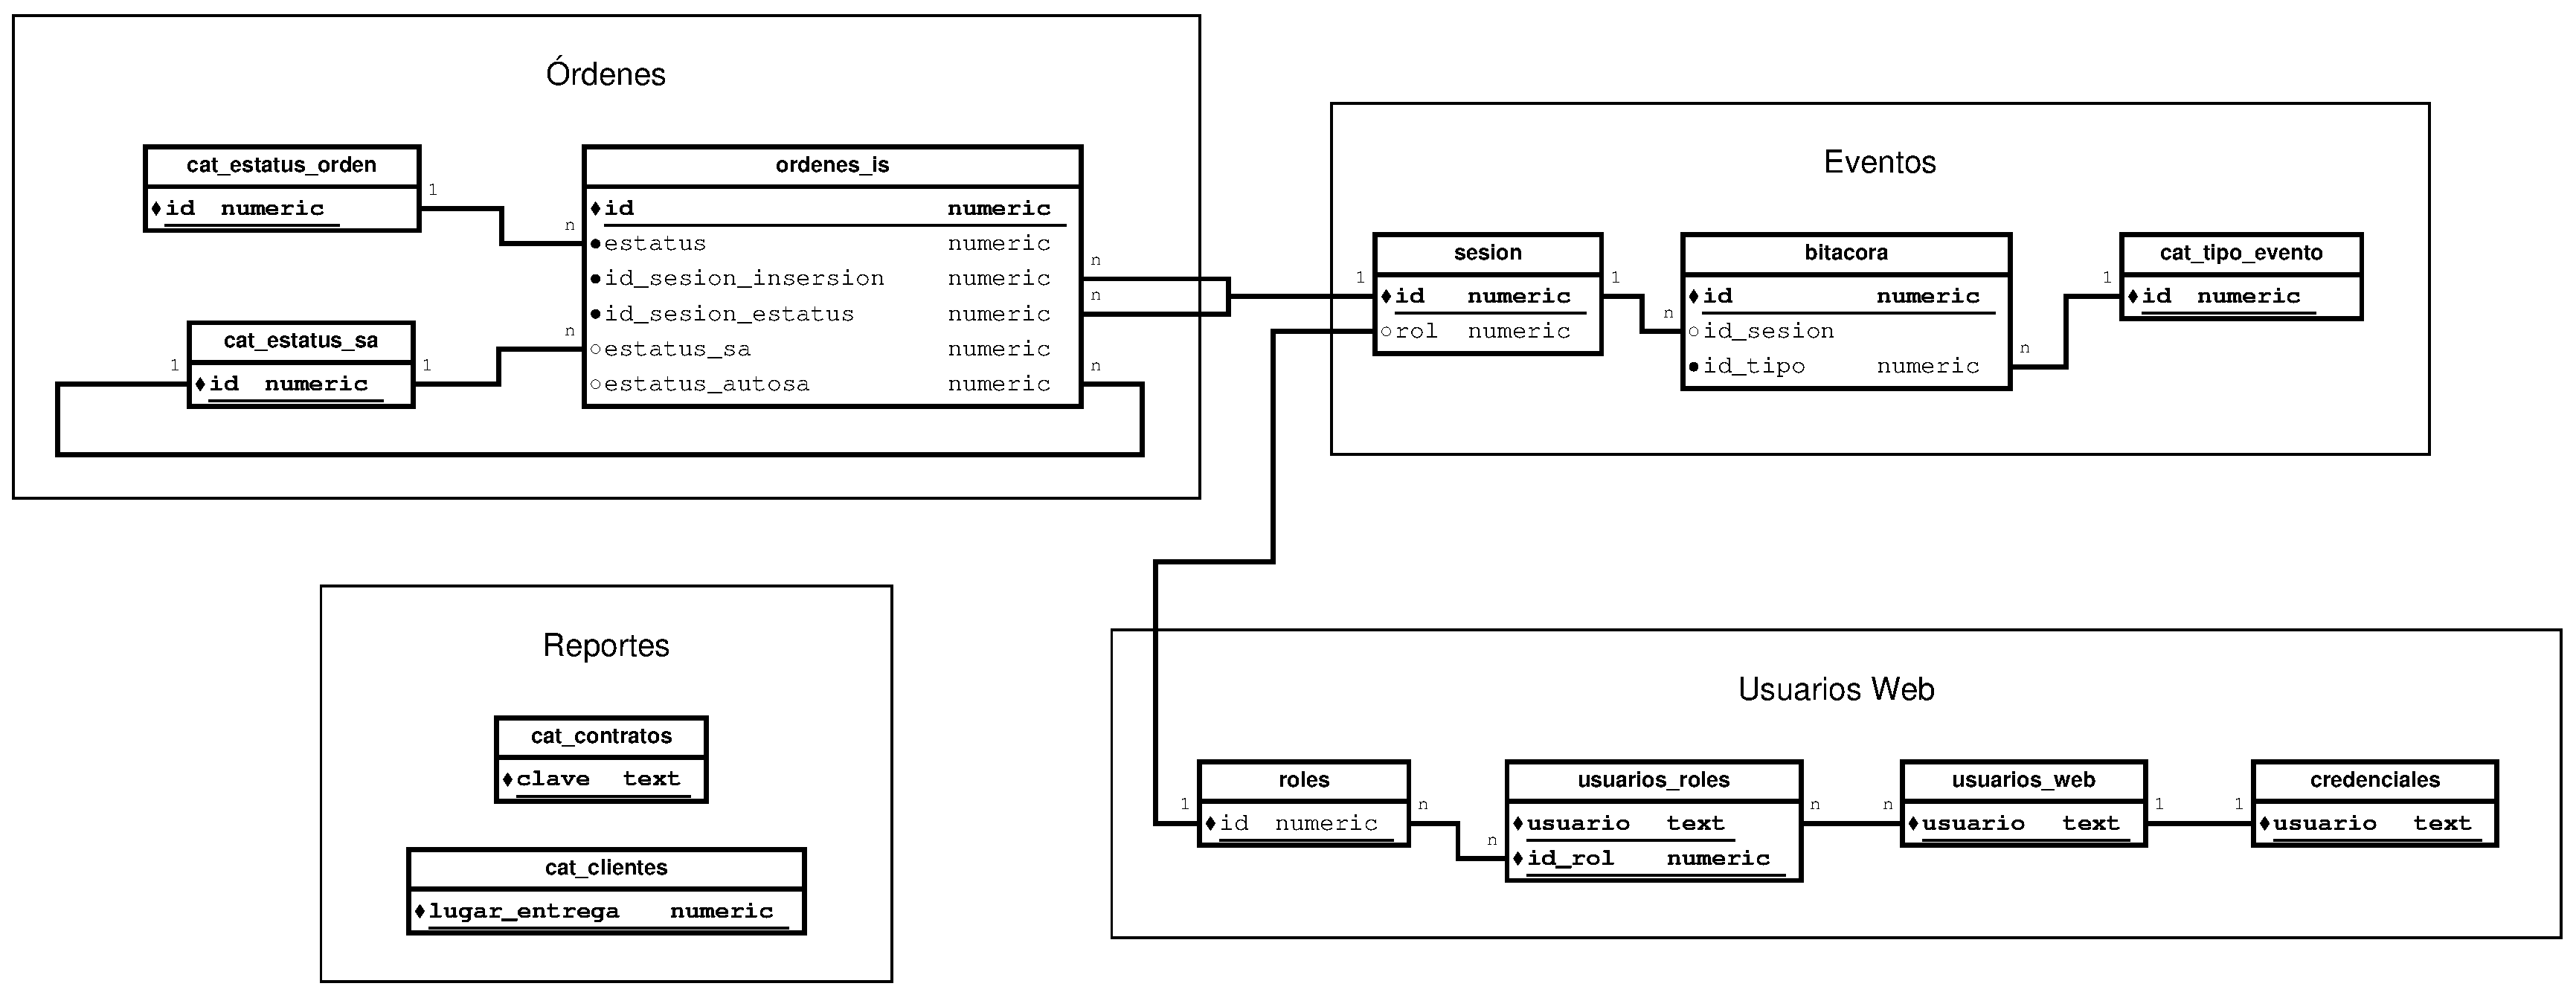
\includegraphics[width=\textwidth]{dia-er-resumen}
  \caption{Diagrama Entidad Relación de el Sistema AutoSA.}
  \label{fig:dia-er-resumen}
\end{figure}

\subsection{Tablas del registro de eventos}
El registro de eventos es todo lo relacionado con actividad de los actores del sistema (robots de automatización y usuarios), como se muestra en la Figura \ref{fig:dia-er-bitacora}.
\begin{figure}[h]
  \centering
  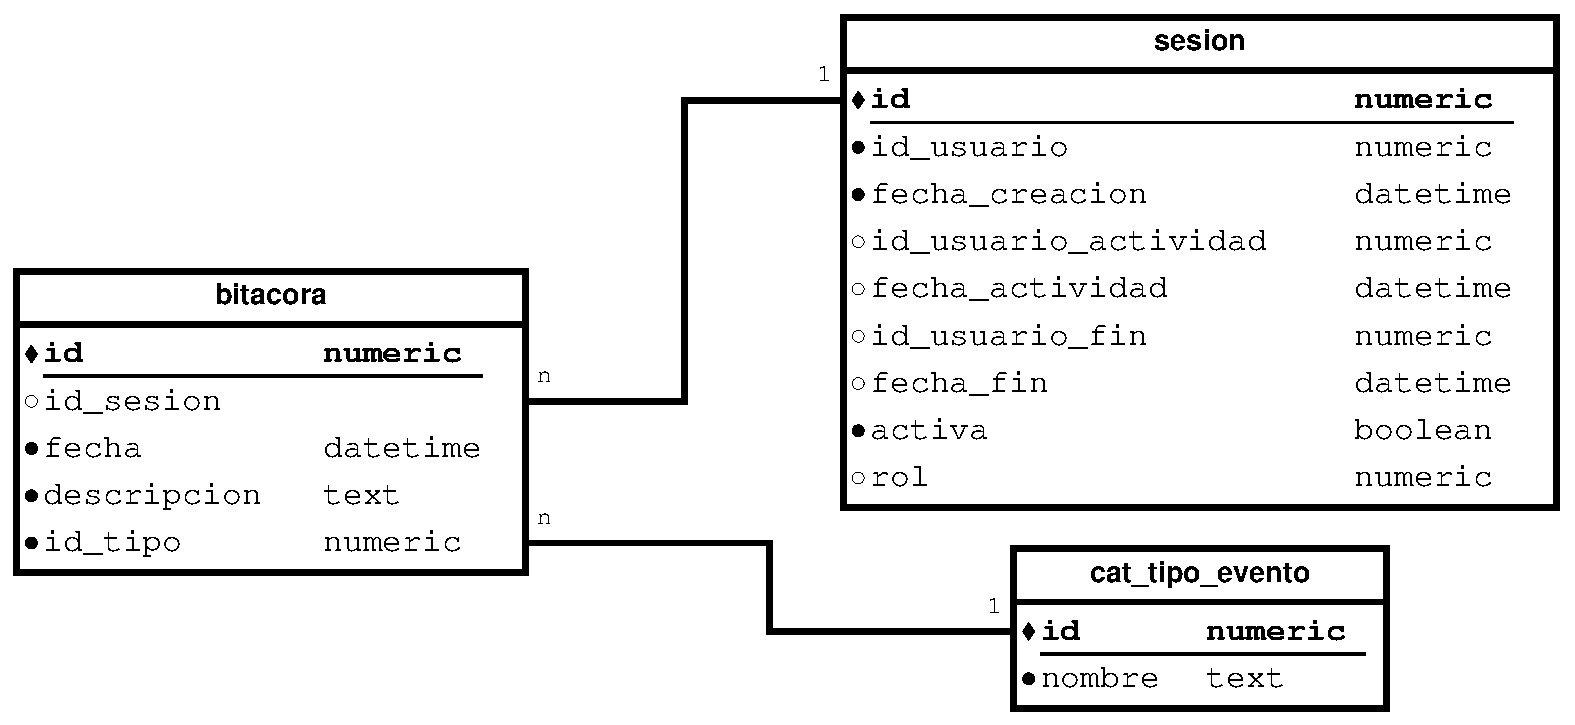
\includegraphics[scale=0.4]{dia-er-bitacora} 
  \caption{Diagrama Entidad Relación para el registro de eventos.}
  \label{fig:dia-er-bitacora}
\end{figure}
\paragraph{bitacora\\} Lleva el registro de eventos ocurridos durante la ejecución de las rutinas de automatización, el evento puede estar ligado a una sesión.
\paragraph{cat{\textunderscore}tipo{\textunderscore}evento\\} Catálogo con los tipos de eventos que pueden ser registrados en la bitácora.
\paragraph{sesion\\} Define una sesión bajo la cual se ejecuta una rutina de automatización, la sesión puede definir implícitamente un usuario y un rol.

\subsection{Tablas de las órdenes de reposición}
En estas tablas (ver Figura \ref{fig:dia-er-ordenes}) se almacenan las órdenes de reposición atendidas durante la rutina automatizada para responder órdenes de reposición en SA\footnote{Ver caso de uso \ref{cu-contestar}}, de igual manera también es utilizada en la verificación de órdenes de reposición canceladas\footnote{Ver caso de uso \ref{cu-verificar}}.
\begin{figure}[h]
  \centering
  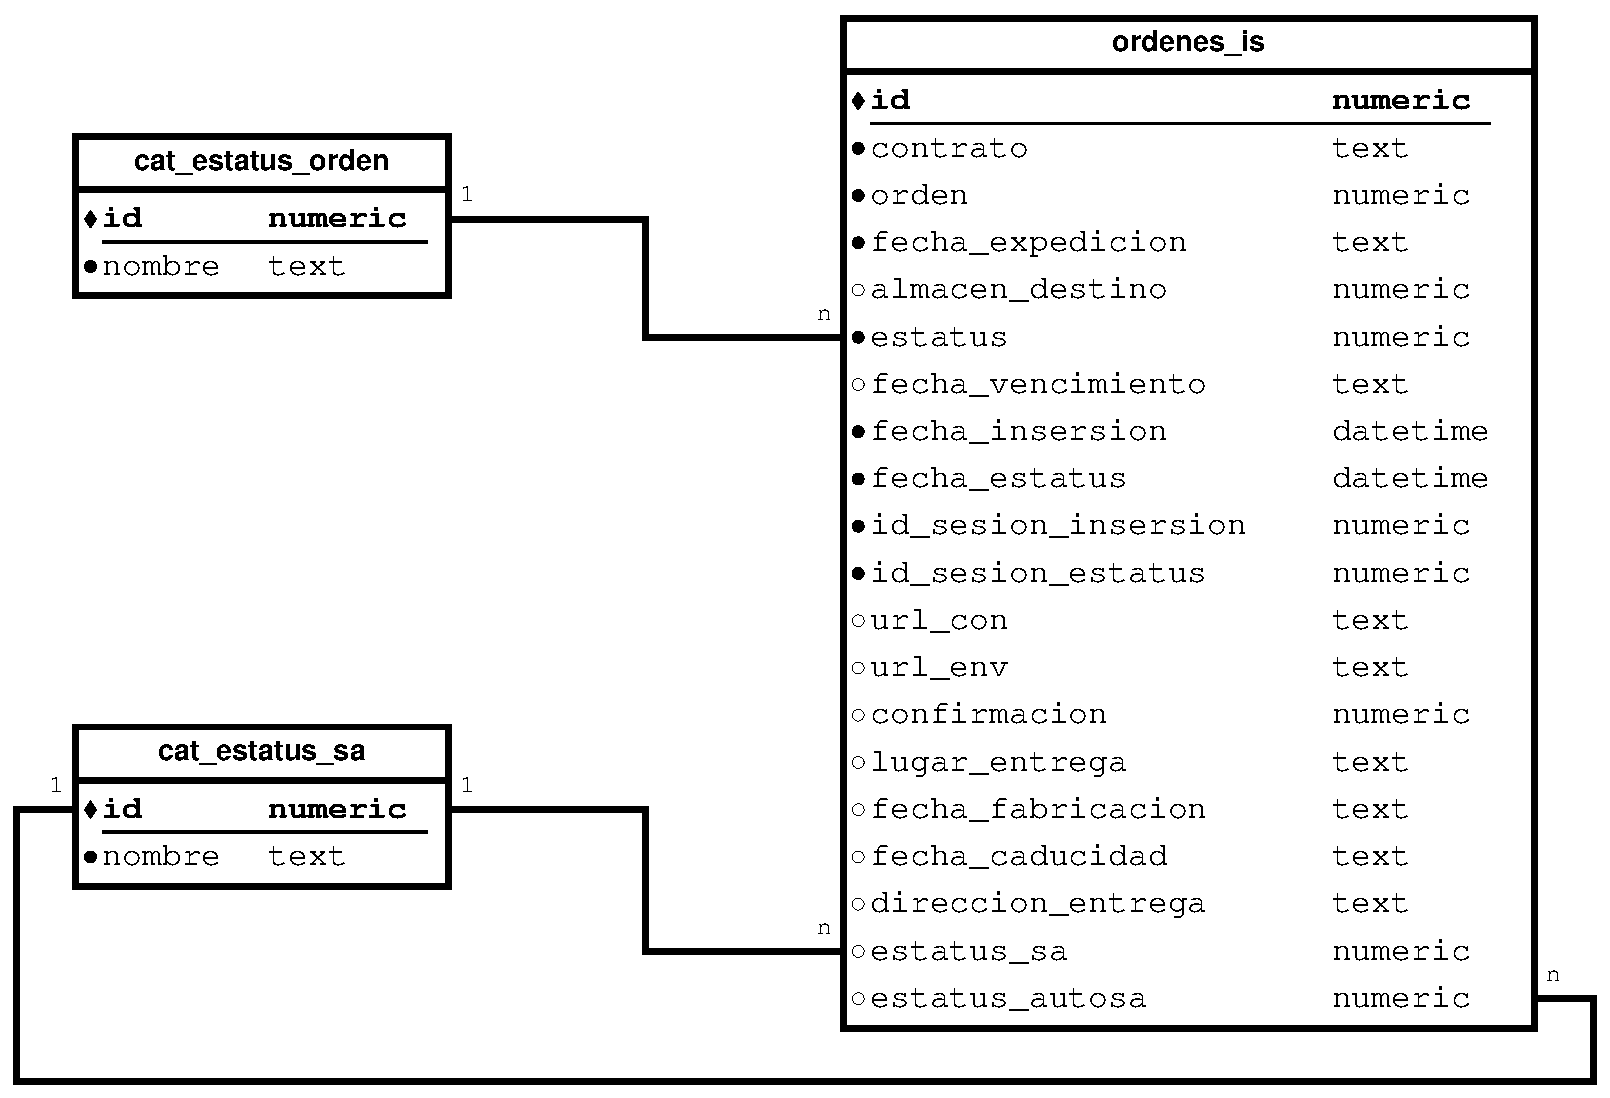
\includegraphics[scale=0.4]{dia-er-ordenes} 
  \caption{Diagrama Entidad Relación para el registro de ordenes de reposición.}
  \label{fig:dia-er-ordenes}
\end{figure}
\paragraph{ordenes{\textunderscore}is\\} Contiene el registro de las órdenes de reposición de SA que han sido atendidas por la rutina de automatización.
\paragraph{cat{\textunderscore}estatus{\textunderscore}orden\\} Este catálogo no debe ser alterado, contiene los posibles estatus que pude tomar una orden durante el ciclo de vida de la aplicación.
\paragraph{cat{\textunderscore}estatus{\textunderscore}sa\\} Este catálogo contiene los estados definidos por SA para una orden de reposición.


\subsection{Tablas de los usuarios de la interfaz web}
Las tablas de este grupo son utilizadas para gestionar el acceso a la interfaz web\footnote{Ver caso de uso \ref{cu-entrar-web}} (ver Figura \ref{fig:dia-er-web}).
\begin{figure}[h]
  \centering
  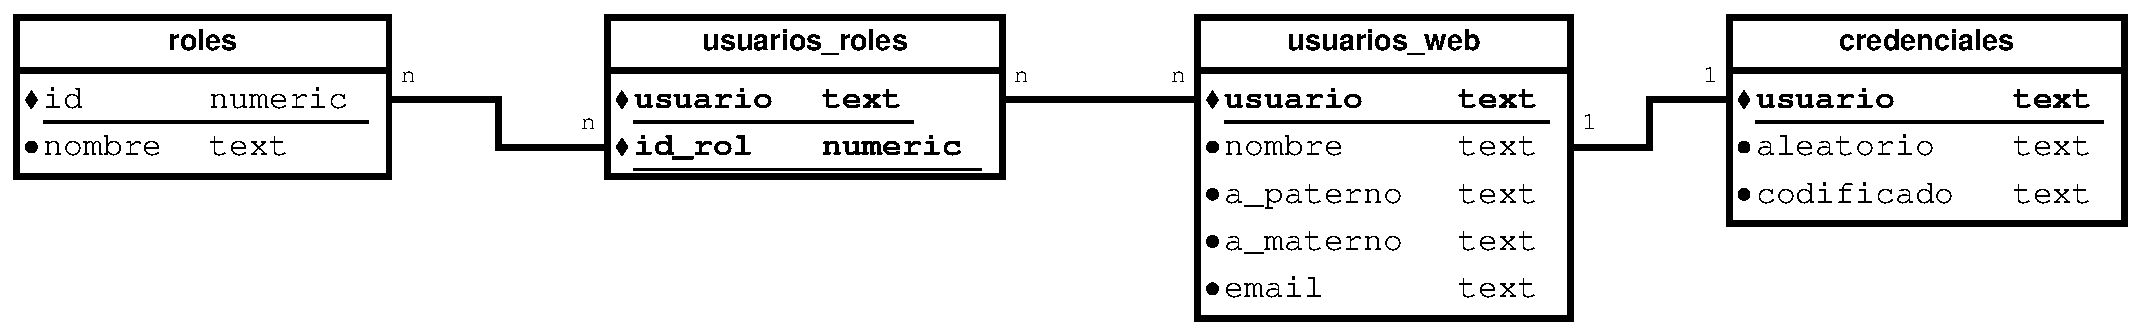
\includegraphics[width=\textwidth]{dia-er-web} 
  \caption{Diagrama Entidad Relación para el manejo de usuarios.}
  \label{fig:dia-er-web}
\end{figure}
\paragraph{roles\\}Contiene los roles (permisos) que los usuarios pueden tener en la interfaz web.
\paragraph{sesion\\}Contiene información de las sesiones de los usuarios de la interfaz web.
\paragraph{usuarios{\textunderscore}web\\} Contiene la información de los usuarios de la interfaz web.
\paragraph{credenciales\\} Contiene la credenciales con las cuales los usuarios autentican su acceso a la interfaz web.


\subsection{Catálogos para la generación de reportes}
Estas tablas contienen catálogos (ver Figura \ref{fig:dia-er-reportes}) que son necesarios para la generación de los reportes\footnote{Ver casos de uso \ref{cu-generar-reporte} y \ref{cu-actualizar-catalogo}} que sirven que las siguientes áreas de la farmacéutica continúen con la atención de las órdenes de reposición.
\begin{figure}[h]
  \centering
  \includegraphics[scale=0.4]{dia-er-reportes} 
  \caption{Diagrama Entidad Relación de los catálogos para la generación de vistas.}
  \label{fig:dia-er-reportes}
\end{figure}
\paragraph{cat{\textunderscore}clientes\\} Este catálogo contiene información sobre la localización física de los lugares donde deben ser entregados los productos.
\paragraph{cat{\textunderscore}contratos\\} Este catálogo contiene información referente a acuerdos comerciales referentes a los productos requeridos en las órdenes de reposición.


%===============================================================================
%===============================================================================
%
%
%\section{Diseño de bibliotecas}
%
%
%===============================================================================
%===============================================================================
%
%
%\section{Diseño de rutinas de automatización}
%
%
%===============================================================================
%===============================================================================
%
%
%\section{Diseño de servicios}
%\subsection{Persistencia}
%\subsection{Acceso y Autorización}
%\subsection{Ordenes de Reposición}
%\subsection{Reportes}
%
%
%===============================================================================
%===============================================================================
%
%
%\section{Diseño de interfaz de usuario}
%
%
